\documentclass[12pt,a4paper]{ctexart}
\usepackage[margin=2.5cm]{geometry}
\usepackage{amsmath,amssymb}
\usepackage{tikz}
\usetikzlibrary{arrows.meta,calc,decorations.pathmorphing,positioning,shapes.symbols}
\setlength{\parindent}{2em}
\setlength{\parskip}{0pt}
\renewcommand{\arraystretch}{1.18}
\title{第35至42届全国中学生物理竞赛复赛\\题干、解析与TikZ图册}
\author{董兴习}
\date{持续建设中}
\begin{document}
\pagestyle{plain}
\maketitle
\tableofcontents

\section*{编制说明}
\addcontentsline{toc}{section}{编制说明}
本图册按大题逐题整理题干、参考解答与题图。原始PDF、OCR与裁图仅作为转写依据；成品不嵌入原题截图。当前仅收录已完成全部文字和图形核对的题目，其他题目以生产清单为准，不以空白页面或未经核实的OCR替代。

% 题干转写：完成
% 解析转写：完成
% 图形核对：完成
\section{第35届复赛第1题：地球引力场中的发射运动}
\subsection{题干}
假设地球为质量分布各向同性的球体。空间站位于地面上方高度 $h$ 处，从站内向与地心连线垂直的方向发射小物体。已知地球半径 $R$、质量 $M$、引力常量 $G$；忽略地球自转与大气影响。
\begin{enumerate}
\item 若物体能绕地球作周期运动，初速度大小应满足什么条件？
\item 若初速度为 $v_0$ 且物体会落到地面，求落地速度大小、速度与水平分量的夹角，以及由发射至落地的时间。
\end{enumerate}

\subsection{参考解答整理}
\paragraph{（1）不落地的周期运动条件。} 初始能量和角动量为
\[
E=\frac12mv_0^2-\frac{GMm}{R+h},\qquad L=mv_0(R+h).
\]
有界运动要求 $E<0$。若椭圆轨道恰好与地面相切，切点速度记为 $v$，则
\[
mv_{0\min}(R+h)=mvR,
\qquad
\frac12mv_{0\min}^2-\frac{GMm}{R+h}
=\frac12mv^2-\frac{GMm}{R}.
\]
解得临界初速度
\[
v_{0\min}=\sqrt{\frac{2GMR}{(R+h)(2R+h)}}.
\]
故物体能作不与地面相交的圆或椭圆轨道运动的条件为
\[
\boxed{\sqrt{\frac{2GMR}{(R+h)(2R+h)}}<v_0<\sqrt{\frac{2GM}{R+h}}.}
\]

\paragraph{（2）落地速度、方向与时间。} 当
\[
v_0<\sqrt{\frac{2GMR}{(R+h)(2R+h)}}
\]
时，轨道与地球表面相交。由机械能守恒，落地速度大小为
\[
v=\sqrt{v_0^2+\frac{2GMh}{R(R+h)}}.
\]
由角动量守恒，落地瞬间的水平分量为
\[
v_\theta=\frac{R+h}{R}v_0.
\]
若 $\alpha$ 为速度与水平分量的夹角，则
\[
\alpha=\arccos\!\left(
\frac{(R+h)v_0}{R\sqrt{v_0^2+\frac{2GMh}{R(R+h)}}}
\right).
\]
以极坐标 $(r,\theta)$ 描述运动，守恒关系为
\[
r^2\frac{d\theta}{dt}=(R+h)v_0,
\]
\[
\frac{dr}{dt}=-\sqrt{-\frac{(R+h)^2v_0^2}{r^2}+\frac{2GM}{r}+v_0^2-\frac{2GM}{R+h}}.
\]
因此下落时间由下列定积分唯一确定：
\[
t=\int_R^{R+h}\frac{r\,dr}
{\sqrt{\left(v_0^2-\frac{2GM}{R+h}\right)r^2+2GMr-(R+h)^2v_0^2}}.
\]
令 $a=-(R+h)^2v_0^2$、$b=2GM$、$c=v_0^2-2GM/(R+h)$，将题给积分公式代入端点即可得到官方解答中的闭式时间表达式；该式在临界速度处取相应极限。

\subsection{转写依据}
题干依据 \texttt{CPHO35-Q01.md}，公式依据 \texttt{CPHO35-Q01\_formula\_check\_v1.csv} 与答案页第6至9页。原题无题图，故本题无TikZ图件。

% 题干转写：完成
% 解析转写：完成
% 图形核对：完成
\section{第35届复赛第2题：弹簧--摩擦阻尼往返运动}
\subsection{题干}
如图\ref{fig:cpho35q02}，劲度系数为 $k$ 的轻弹簧左端固定、右端连一质量为 $m$ 的小球。弹簧自然状态时小球位于原点 $O$；小球在粗糙水平面上滑动，动摩擦因数为 $\mu$，最大静摩擦力等于滑动摩擦力。初始时小球静止，弹簧伸长为 $-A_0$，其中 $A_0>0$，重力加速度为 $g$。
\begin{figure}[htbp]\centering
\begin{tikzpicture}[>=Stealth,scale=0.9]
  \draw[thick] (-4.4,0) -- (4.6,0);
  \foreach \x in {-4.2,-3.9,...,4.4} {\draw[gray] (\x,0) -- +(0.18,-0.13);}
  \draw[->,thick] (-4.1,0.36) -- (4.25,0.36) node[right] {$x$};
  \draw[thick] (-3.8,-0.55) -- (-3.8,1.25);
  \foreach \y in {-0.45,-0.15,...,1.15} {\draw[thick] (-4.08,\y) -- (-3.8,\y+0.15);}
  \draw[thick,decorate,decoration={coil,segment length=4pt,amplitude=3pt}]
    (-3.8,0.65) -- (-1.15,0.65);
  \fill[blue!25] (-0.82,0.33) rectangle (-0.17,0.98);
  \draw[thick] (-0.82,0.33) rectangle (-0.17,0.98);
  \node at (-0.50,0.66) {$m$};
  \draw[densely dashed] (-0.50,0.1) -- (-0.50,1.1);
  \draw[densely dashed] (1.15,0.1) -- (1.15,1.1);
  \node[below] at (-0.50,0.1) {$-A_0$};
  \node[below] at (1.15,0.1) {$O$};
  \node[above] at (-0.50,1.08) {$t=0$};
  \node[below] at (-2.45,-0.5) {劲度系数 $k$ 的轻弹簧};
\end{tikzpicture}

\caption{第35届复赛第2题题图的TikZ重绘：初始压缩状态、原点和水平坐标轴。}\label{fig:cpho35q02}
\end{figure}
\begin{enumerate}
\item 小球至多只能向右运动时，求最终位置及 $A_0$ 条件；
\item 小球第一次向右越过原点后至多只能向左运动时，求最终位置及条件；
\item 小球只能完成 $n$ 次往返运动时，求最终位置及条件；
\item 在只能完成 $n$ 次往返运动时，求全过程总路程。
\end{enumerate}

\subsection{参考解答整理}
记 $q=\mu mg/k$。每一次由静止位置到下一静止位置的过程中，功能原理给出弹簧势能减少等于摩擦耗散。

\paragraph{（1）至多向右运动。} 若 $0<A_0\leq q$，初始弹力不足以克服静摩擦，小球停在 $x=-A_0$。若 $A_0>q$，第一次向右停下的位置为
\[x=A_0-2q.\]
因此在“至多向右运动”的范围内，最终位置分段为
\[
x=\begin{cases}
-A_0,&0<A_0\leq q,\\
A_0-2q,&q<A_0\leq2q,\\
A_0-2q,&2q<A_0\leq3q.
\end{cases}
\]
第二、三段分别落在原点左侧（或原点）和右侧；其后均因回复弹力不超过 $\mu mg$ 而静止。

\paragraph{（2）至多向左运动。} 当 $3q<A_0\leq4q$ 时，第一次向左停下后仍在原点右侧或原点：
\[x=4q-A_0\geq0.\]
当 $4q<A_0\leq5q$ 时，最终停在原点左侧：
\[x=4q-A_0=-A_1<0.\]

\paragraph{（3）完成 $n$ 次往返后的最终位置。} 令第 $n$ 次返回原点左侧的静止位置为 $-A_n$。相邻转折点的伸长量依次相差 $2q$，故
\[A_n=A_0-4nq.\]
最终位置的完整分段为
\[
x=\begin{cases}
4nq-A_0,&4nq<A_0\leq(4n+1)q,\\
A_0-2(2n+1)q,&(4n+1)q<A_0\leq2(2n+1)q,\\
A_0-2(2n+1)q,&2(2n+1)q<A_0\leq(4n+3)q,\\
4(n+1)q-A_0,&(4n+3)q<A_0\leq4(n+1)q.
\end{cases}
\]
其中第二、四段的右端点分别包含原点情形。

\paragraph{（4）总路程。} 从初态到最终静止位置 $x$ 的能量关系为
\[\frac12kA_0^2-\frac12kx^2=\mu mgs,\qquad s=\frac{k}{2\mu mg}(A_0^2-x^2).\]
代入上述分段终点，得到
\[
s=\begin{cases}
4n(A_0-2nq),&4nq<A_0\leq(4n+1)q,\\
2(2n+1)\bigl[A_0-(2n+1)q\bigr],&(4n+1)q<A_0\leq(4n+3)q,\\
4(n+1)\bigl[A_0-2(n+1)q\bigr],&(4n+3)q<A_0\leq4(n+1)q.
\end{cases}
\]

\subsection{转写依据}
题干、答案分段和题图分别依据 \texttt{CPHO35-Q02.md}、\texttt{CPHO35-Q02\_formula\_check\_v1.csv} 及图件核对入口。分值边界未在当前PDF中明示，未写入本条目。

% 题干转写：完成
% 解析转写：完成
% 图形核对：完成
\section{第35届复赛第3题：细杆打击中心与撤轴后运动}
\subsection{题干}
质量为 $M$、长度为 $l$ 的匀质细杆 $AB$ 自由悬挂于通过原点 $O$ 的水平光滑转轴上，初始时杆竖直下垂。质量为 $m$ 的弹丸以速度 $v_0$ 水平撞击杆的打击中心并嵌入杆中；杆转过半圈恢复竖直状态时立即撤去转轴。忽略地面高度限制，重力加速度为 $g$。如图\ref{fig:cpho35q03}，求打击中心、撤轴前轴力、撤轴后杆端坐标，以及杆再转半圈时 $O,B$ 两点的高度差。
\begin{figure}[htbp]\centering
\begin{tikzpicture}[>=Stealth,scale=0.82]
  \begin{scope}
    \draw[->,thick] (-2.3,0) -- (2.3,0) node[right] {$x$};
    \draw[->,thick] (0,-2.9) -- (0,1.0) node[above] {$y$};
    \fill (0,0) circle (1.5pt) node[above left] {$O$};
    \draw[very thick] (0,0) -- (0,-2.35);
    \node[left] at (-0.10,-1.2) {$M,l$};
    \fill (0,-2.35) circle (1.3pt) node[right] {$B$};
    \draw[->,very thick,red!75!black] (2.0,-1.58) -- (0.72,-1.58) node[midway,above] {$v_0$};
    \fill[blue!65] (0.60,-1.58) circle (3pt) node[right] {$m$};
    \draw[densely dashed] (0,-1.58) -- (0.55,-1.58);
    \node[left] at (-0.1,-1.58) {$L=2l/3$};
    \node[below] at (0,-3.12) {初始撞击状态};
  \end{scope}
  \begin{scope}[xshift=6.0cm]
    \draw[->,thick] (0,0) -- (2.7,0) node[right] {$x'$};
    \draw[->,thick] (0,0) -- (0,2.2) node[above] {$y'$};
    \fill (0,0) circle (1.4pt) node[below left] {质心};
    \draw[very thick] (0,0) -- (1.35,1.35);
    \fill (1.35,1.35) circle (1.2pt) node[above right] {$B$};
    \draw[->,thick,purple!75!black] (0.48,0.48) arc[start angle=45,end angle=-20,radius=0.68];
    \node[purple!75!black] at (0.93,0.15) {$\omega't$};
    \node[below] at (0,-0.55) {撤轴后相对质心转动};
  \end{scope}
\end{tikzpicture}

\caption{第35届复赛第3题题图与撤轴后相对质心坐标的TikZ重绘。}\label{fig:cpho35q03}
\end{figure}

\subsection{参考解答整理}
\paragraph{（1）打击中心。} 设作用点到 $O$ 的距离为 $L$。由杆绕端点的转动方程与质心平动关系，
\[FL=\frac13Ml^2\beta,\qquad F-F_x=Ma_x,\qquad a_x=\frac l2\beta.\]
打击中心要求撞击瞬间 $F_x=0$，故
\[\boxed{L=\frac23l.}\]

\paragraph{（2）撤轴前的轴力。} 碰撞后杆--弹丸系统的质心到轴距离、初始角速度和转动惯量为
\[
L_c=\frac{4m+3M}{6(M+m)}l,\qquad
\omega_0=\frac{6mv_0}{(4m+3M)l},\qquad
I=\frac19(3M+4m)l^2.
\]
转过 $\theta$ 后，机械能守恒给出
\[
\omega^2=\frac{36m^2v_0^2}{(4m+3M)^2l^2}-\frac{3g}{l}(1-\cos\theta),
\qquad \beta'=\frac{3g}{2l}\sin\theta.
\]
轴对系统作用力的分量为
\[
N_x=\frac{(4m+3M)g}{4}(3\sin\theta\cos\theta-2\sin\theta)
+\frac{6m^2v_0^2}{(4m+3M)l}\sin\theta,
\]
\[
N_y=(M+m)g+\frac{6m^2v_0^2}{(4m+3M)l}\cos\theta
+\frac{(4m+3M)g}{4}(3\cos^2\theta-2\cos\theta-1).
\]

\paragraph{（3）撤轴后的杆端轨迹。} 在 $\theta=\pi$ 时撤轴，角速度记为
\[
\omega'=\sqrt{\frac{36m^2v_0^2}{(4m+3M)^2l^2}-\frac{6g}{l}}.
\]
此后质心作平抛、杆绕质心顺时针转动。以撤轴瞬间为 $t=0$，杆端 $B$ 的坐标为
\[
x_B(t)=L_c\omega't+(l-L_c)\sin(\omega't),
\]
\[
y_B(t)=L_c-\frac12gt^2+(l-L_c)\cos(\omega't).
\]

\paragraph{（4）再转半圈时的高度差。} 令 $\omega't_1=\pi$，则
\[
h=\left|2L_c-l-\frac12g\left(\frac\pi{\omega'}\right)^2\right|
=\left|\frac{\pi^2g}{2}\left[\frac{36m^2v_0^2}{(4m+3M)^2l^2}-\frac{6g}{l}\right]^{-1}-\frac{ml}{3(M+m)}\right|.
\]

\subsection{转写依据}
题干、答案公式和题图分别依据 \texttt{CPHO35-Q03.md}、\texttt{CPHO35-Q03\_formula\_check\_v1.csv} 及图件核对入口；当前PDF未明示分值，未写入图册。

% 题干转写：完成
% 解析转写：完成
% 图形核对：完成
\section{第35届复赛第4题：Ioffe--Pritchard 磁阱}
\subsection{题干}
四根通有恒定电流 $I$ 的长直导线垂直于 $x$--$y$ 平面，其与该平面的交点构成边长为 $2a$、中心为原点 $O$ 的正方形顶点。导线 $1,2,3,4$ 的坐标依次为 $(-a,a)$、$(a,a)$、$(a,-a)$、$(-a,-a)$，电流方向如图\ref{fig:cpho35q04}。装置还置于匀强磁场 $\boldsymbol B_0=B_0\boldsymbol k$ 中，$\boldsymbol k$ 为 $z$ 轴正方向单位矢量，真空磁导率为 $\mu_0$。

求：（1）四根导线在导线外产生的总磁场空间分布；（2）原点附近保留线性项的总磁场；（3）若原子的束缚势能 $V=\mu\lvert\boldsymbol B_{\mathrm{tot}}\rvert$，其中 $\mu>0$，求原点附近的磁场力；（4）原子最易从 $x$--$y$ 平面的何处逸出，并求刚好逸出的动能。
\begin{figure}[htbp]\centering
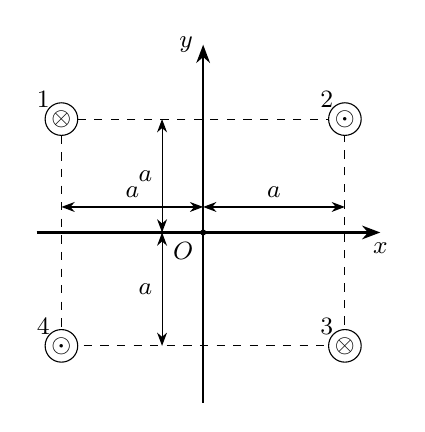
\begin{tikzpicture}[scale=0.9,>=Stealth,font=\small]
  \draw[->,thick] (-0.35,0) -- (4.5,0) node[below] {$x$};
  \draw[->,thick] (2,-2.4) -- (2,2.65) node[left] {$y$};
  \draw[dashed] (0,1.6) rectangle (4,-1.6);
  \coordinate (O) at (2,0);
  \foreach \x/\y/\lab/\sym in {0/1.6/1/$\otimes$,4/1.6/2/$\odot$,4/-1.6/3/$\otimes$,0/-1.6/4/$\odot$}{
    \draw[fill=white] (\x,\y) circle (0.23);
    \node at (\x,\y) {\sym};
    \node[above left=1pt] at (\x,\y) {\lab};
  }
  \fill (O) circle (1.2pt) node[below left] {$O$};
  \draw[<->] (0,0.36) -- (2,0.36) node[midway,above] {$a$};
  \draw[<->] (2,0.36) -- (4,0.36) node[midway,above] {$a$};
  \draw[<->] (1.42,0) -- (1.42,1.6) node[midway,left] {$a$};
  \draw[<->] (1.42,-1.6) -- (1.42,0) node[midway,left] {$a$};
\end{tikzpicture}

\caption{第35届复赛第4题 Ioffe--Pritchard 磁阱的 TikZ 重绘。$\otimes$ 表示电流垂直纸面向里，$\odot$ 表示电流垂直纸面向外。}\label{fig:cpho35q04}
\end{figure}

\subsection{参考解答整理}
\paragraph{（1）四导线磁场的叠加。} 取 $x$、$y$ 方向单位矢量为 $\boldsymbol i$、$\boldsymbol j$。导线外任一点 $(x,y)$ 处，四根导线分别产生
\[
\begin{aligned}
\boldsymbol B_1&=\frac{\mu_0(-I)}{2\pi}\frac{-(y-a)\boldsymbol i+(x+a)\boldsymbol j}{(x+a)^2+(y-a)^2},&
\boldsymbol B_2&=\frac{\mu_0 I}{2\pi}\frac{-(y-a)\boldsymbol i+(x-a)\boldsymbol j}{(x-a)^2+(y-a)^2},\\
\boldsymbol B_3&=\frac{\mu_0(-I)}{2\pi}\frac{-(y+a)\boldsymbol i+(x-a)\boldsymbol j}{(x-a)^2+(y+a)^2},&
\boldsymbol B_4&=\frac{\mu_0 I}{2\pi}\frac{-(y+a)\boldsymbol i+(x+a)\boldsymbol j}{(x+a)^2+(y+a)^2}.
\end{aligned}
\]
因此导线电流产生的总磁场为
\[
\boldsymbol B=\boldsymbol B_1+\boldsymbol B_2+\boldsymbol B_3+\boldsymbol B_4.
\]

\paragraph{（2）原点附近的线性近似。} 在 $|x|\ll a$、$|y|\ll a$ 的范围内，将上式保留至 $x/a$、$y/a$ 的一次项，得到
\[
\boxed{\boldsymbol B\simeq\frac{\mu_0I}{\pi a^2}\left(x\boldsymbol i-y\boldsymbol j\right).}
\]
加上沿 $z$ 轴的偏置磁场后，
\[
\boldsymbol B_{\mathrm{tot}}\simeq\frac{\mu_0I}{\pi a^2}\left(x\boldsymbol i-y\boldsymbol j\right)+B_0\boldsymbol k.
\]

\paragraph{（3）原点附近的束缚力。} 磁感应强度大小的二阶展开为
\[
\lvert\boldsymbol B_{\mathrm{tot}}\rvert
=\sqrt{B_0^2+\left(\frac{\mu_0I}{\pi a^2}\right)^2(x^2+y^2)}
\simeq B_0+\frac{1}{2B_0}\left(\frac{\mu_0I}{\pi a^2}\right)^2(x^2+y^2).
\]
于是势能及其负梯度为
\[
V\simeq\mu B_0+\frac{\mu}{2B_0}\left(\frac{\mu_0I}{\pi a^2}\right)^2(x^2+y^2),
\qquad
\boxed{\boldsymbol F=-\frac{\mu}{B_0}\left(\frac{\mu_0I}{\pi a^2}\right)^2(x\boldsymbol i+y\boldsymbol j).}
\]
该力在 $x$--$y$ 平面内沿径向指向原点。

\paragraph{（4）逸出位置与阈值动能。} 完整势能可写为
\[
V=\mu\sqrt{B_0^2+\lvert\boldsymbol B\rvert^2}.
\]
在 $x$ 轴上取 $y=0$，有
\[
V(x,0)=\mu\sqrt{B_0^2+\left(\frac{\mu_0Ia}{\pi}\right)^2
\left[\frac{1}{(x-a)^2+a^2}-\frac{1}{(x+a)^2+a^2}\right]^2}.
\]
由 $\mathrm dV/\mathrm dx=0$ 得 $x(3x^4-4a^4)=0$。原点为势能最小点；势垒顶点位于
\[
\boxed{\left(\pm\left(\frac43\right)^{1/4}a,0\right),\qquad
\left(0,\pm\left(\frac43\right)^{1/4}a\right).}
\]
这些点给出原子在平面内最易逸出的四个方向。势垒高度对应的势能为
\[
V_{\mathrm b}=\mu\sqrt{B_0^2+\frac{3\sqrt3}{8}\left(\frac{\mu_0I}{\pi a}\right)^2},
\qquad V_O=\mu B_0.
\]
故刚好逸出磁阱所需的最小动能为
\[
\boxed{E_k=\mu B_0\left[\sqrt{1+\frac{3\sqrt3}{8}\left(\frac{\mu_0I}{\pi aB_0}\right)^2}-1\right].}
\]

\subsection{转写依据}
题干、答案公式和题图分别依据 \texttt{CPHO35-Q04.md}、\texttt{CPHO35-Q04\_formula\_check\_v1.csv} 及图件核对入口；当前PDF未明示分值，未写入图册。

% 题干转写：完成
% 解析转写：完成
% 图形核对：完成
\section{第35届复赛第5题：塞曼效应的经典解释}
\subsection{题干}
钠光 $D$ 线在磁场中会分裂为三条。设原子中的价电子质量为 $m$、电荷量为 $-e$（$e>0$），受到指向原子中心的等效线性回复力
\[
\boldsymbol F_{\mathrm r}=-m\omega_0^2\boldsymbol r,
\]
其中 $\boldsymbol r$ 是电子相对于原子中心的位矢。电子的固有圆频率为 $\omega_0$。现加一沿 $z$ 轴正方向的匀强磁场，磁感应强度参数化为
\[
B=\frac{2m}{e}\omega_L.
\]
求：（1）选择绕磁场方向匀角速转动的参考系，使电子在该系中作简谐运动，导出直角坐标分量方程及其解；（2）将该解变换回实验室参考系；（3）证明原来圆频率为 $\omega_0$ 的谱线分裂为三条，并求弱磁场 $\omega_L\ll\omega_0$ 时相邻谱线的圆频率间隔。已知转动参考系中的科里奥利力为 $\boldsymbol f_{\mathrm c}=-2m\boldsymbol\omega\times\boldsymbol v'$。

\subsection{参考解答整理}
\paragraph{（1）旋转参考系中的简谐运动。} 实验室系中电子满足
\[
m\boldsymbol a=-m\omega_0^2\boldsymbol r-e\boldsymbol v\times\boldsymbol B.
\]
取绕 $z$ 轴转动的参考系 $Ox'y'z'$，并令其角速度为
\[
\boldsymbol\omega=\omega_L\boldsymbol k'.
\]
利用 $\boldsymbol r=\boldsymbol r'$、$\boldsymbol v=\boldsymbol\omega\times\boldsymbol r'+\boldsymbol v'$，离心力和科里奥利力中的速度耦合项相消。电子在旋转系中满足
\[
\ddot x'=-(\omega_0^2+\omega_L^2)x',\qquad
\ddot y'=-(\omega_0^2+\omega_L^2)y',\qquad
\ddot z'=-\omega_0^2z'.
\]
记
\[
\Omega=\sqrt{\omega_0^2+\omega_L^2},
\]
则一般解可写为
\[
x'=A_1\cos(\Omega t+\varphi_1),\qquad
y'=A_2\sin(\Omega t+\varphi_2),\qquad
z'=A_3\cos(\omega_0t+\varphi_3).
\]

\paragraph{（2）变换回实验室系。} 两坐标系之间的旋转变换为
\[
x=x'\cos\omega_Lt-y'\sin\omega_Lt,\qquad
y=x'\sin\omega_Lt+y'\cos\omega_Lt,\qquad z=z'.
\]
将旋转系解代入后，以积化和差公式合并同频项，实验室系中的运动可整理为
\[
\begin{aligned}
x&=A_+\cos(\omega_+t+\varphi_+)+A_-\cos(\omega_-t+\varphi_-),\\
y&=A_+\sin(\omega_+t+\varphi_+)-A_-\sin(\omega_-t+\varphi_-),\\
z&=A_3\cos(\omega_0t+\varphi_3),
\end{aligned}
\]
其中
\[
\boxed{\omega_\pm=\sqrt{\omega_0^2+\omega_L^2}\pm\omega_L.}
\]

\paragraph{（3）谱线分裂与弱场极限。} 上式表明电子的振动包含 $\omega_+$、$\omega_0$、$\omega_-$ 三个圆频率，因此原来的谱线在磁场中分裂为三条。弱磁场条件下，
\[
\sqrt{\omega_0^2+\omega_L^2}
=\omega_0+O\!\left(\frac{\omega_L^2}{\omega_0}\right),
\]
从而
\[
\omega_\pm\simeq\omega_0\pm\omega_L,\qquad
\boxed{\omega_+-\omega_0=\omega_0-\omega_-=\omega_L.}
\]

\subsection{转写依据}
题干、答案公式分别依据 \texttt{CPHO35-Q05.md} 和 \texttt{CPHO35-Q05\_formula\_check\_v1.csv}。原题无题图，故本题无TikZ图件；当前PDF未明示分值，未写入图册。

% 题干转写：完成
% 解析转写：完成
% 图形核对：完成
\section{第35届复赛第6题：同心球壳辐射与导热}
\subsection{题干}
如图\ref{fig:cpho35q06}，太空中有一由同心内球和球壳构成的实验装置，二者之间为真空。内球半径 $r=0.200\,\mathrm m$、比辐射率 $e=0.800$、温度恒定；球壳导热系数 $\kappa=1.00\times10^{-2}\,\mathrm{J\,m^{-1}\,s^{-1}\,K^{-1}}$，内、外半径分别为 $R_1=0.900\,\mathrm m$、$R_2=1.00\,\mathrm m$。球壳内表面比辐射率为 $E=0.800$，外表面视为黑体。斯特藩常量 $\sigma=5.67\times10^{-8}\,\mathrm{W\,m^{-2}\,K^{-4}}$，宇宙微波背景温度 $T=2.73\,\mathrm K$。热稳定时，球壳内表面传给外表面的热量为 $Q=44.0\,\mathrm W$。

求：（1）球壳外表面温度 $T_2$；（2）球壳内表面温度 $T_1$；（3）内球温度 $T_0$。
\begin{figure}[htbp]\centering
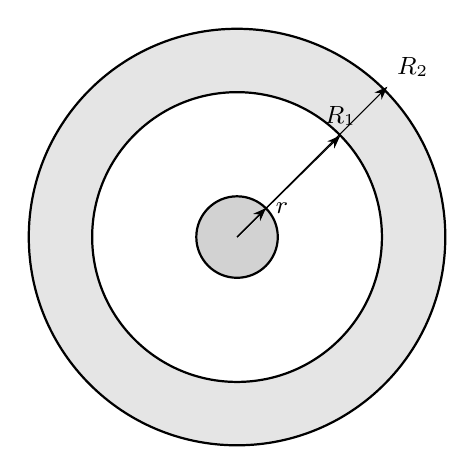
\begin{tikzpicture}[scale=1.15,>=Stealth,font=\small]
  \fill[gray!20,even odd rule] (0,0) circle (2.3) (0,0) circle (1.6);
  \draw[thick] (0,0) circle (2.3);
  \draw[thick] (0,0) circle (1.6);
  \fill[gray!35] (0,0) circle (0.45);
  \draw[thick] (0,0) circle (0.45);
  \draw[->] (0,0) -- (0.32,0.32);
  \node[right] at (0.32,0.32) {$r$};
  \draw[->] (0,0) -- (1.14,1.12);
  \node[above] at (1.14,1.12) {$R_1$};
  \draw[->] (0,0) -- (1.66,1.66);
  \node[above right] at (1.66,1.66) {$R_2$};
\end{tikzpicture}

\caption{第35届复赛第6题同心内球与球壳的 TikZ 重绘。}\label{fig:cpho35q06}
\end{figure}

\subsection{参考解答整理}
\paragraph{（1）球壳外表面温度。} 外表面为黑体，向背景辐射的净功率为
\[
Q'=4\pi R_2^2\sigma(T_2^4-T^4).
\]
热稳定时 $Q'=Q$，故
\[
T_2=\left(\frac{Q}{4\pi R_2^2\sigma}+T^4\right)^{1/4}
=\boxed{88.6\,\mathrm K}.
\]

\paragraph{（2）球壳内表面温度。} 半径为 $R$ 的球面上通过的导热功率恒为 $Q$。由傅里叶热传导定律，
\[
Q=-4\pi R^2\kappa\frac{\mathrm dT}{\mathrm dR}.
\]
将 $R:R_1\to R_2$、$T:T_1\to T_2$ 积分，得
\[
Q=4\pi\kappa\frac{R_1R_2}{R_2-R_1}(T_1-T_2),
\]
\[
T_1=T_2+\frac{(R_2-R_1)Q}{4\pi\kappa R_1R_2}
=\boxed{128\,\mathrm K}.
\]

\paragraph{（3）内球温度。} 内球表面积为 $S_{\mathrm I}=4\pi r^2$，球壳内表面积为 $S_{\mathrm{II}}=4\pi R_1^2$。球壳内表面向内反射的辐射中，能重新到达内球的几何份额为
\[
k=\left(\frac{r}{R_1}\right)^2.
\]
将内球与球壳内表面之间的多次反射和吸收写为几何级数并求和，内球传给球壳的净辐射功率为
\[
Q''=\frac{4\pi Ee\sigma r^2(T_0^4-T_1^4)}
{1-(1-e)k(1-E)}.
\]
热稳定给出 $Q''=Q$，于是
\[
T_0=
\left\{
\frac{\left[1-(1-e)(1-E)\dfrac{r^2}{R_1^2}\right]Q}
{4\pi Ee\sigma r^2}
+T_1^4
\right\}^{1/4}
=\boxed{227\,\mathrm K}.
\]

\subsection{转写依据}
题干、答案公式和题图分别依据 \texttt{CPHO35-Q06.md}、\texttt{CPHO35-Q06\_formula\_check\_v1.csv} 及题图核对入口；当前PDF未明示分值，未写入图册。

% 题干转写：完成
% 解析转写：完成
% 图形核对：完成
\section{第35届复赛第7题：弹簧衍射与DNA X射线衍射类比}
\subsection{题干}
用波长 $\lambda=633\,\mathrm{nm}$ 的激光水平照射竖直圆珠笔中的小弹簧，在距离弹簧 $L=4.2\,\mathrm m$ 的光屏上形成衍射图像，如图\ref{fig:cpho35q07}（a）。该图像与用波长 $\lambda'=0.15\,\mathrm{nm}$ 的平行X射线照射DNA样品、在距离 $L'=9.0\,\mathrm{cm}$ 的底片上获得的图\ref{fig:cpho35q07}（b）相似。

求：（1）利用图（a）的尺寸信息估算弹簧钢丝直径 $d_1$、弹簧半径 $R$ 和螺距 $p$；（2）利用图（b）的尺寸信息估算DNA螺旋半径 $R'$ 和螺距 $p'$。已知两段互成角度的细铁丝的衍射干涉图像，与两条成同样角度、相同宽度的狭缝图像一致。
\begin{figure}[htbp]\centering
\begin{tikzpicture}[>=Stealth,font=\small]
  % 图a：弹簧与交叉衍射条纹
  \begin{scope}
    \node[font=\bfseries] at (1.9,3.65) {（a）弹簧与激光衍射图样};
    \draw[thick] (0.5,0.4) -- (0.5,3.0);
    \draw[thick,domain=0:720,samples=180,smooth,variable=\t]
      plot ({1.05+0.30*sin(\t)}, {0.55+\t/300});
    \draw[thick] (1.55,0.4) -- (1.55,3.0);
    \node[below] at (1.03,0.35) {弹簧};
    \draw[fill=black] (3.35,0.45) rectangle (5.75,3.0);
    \foreach \yy in {0.72,0.98,1.24,1.50,1.76,2.02,2.28,2.54,2.80}{
      \draw[red!75!yellow,line width=1.2pt] (4.55,\yy) -- (3.55,{0.53+0.47*(\yy-0.55)}) -- (3.72,{0.53+0.47*(\yy-0.55)});
      \draw[red!75!yellow,line width=1.2pt] (4.55,\yy) -- (5.55,{0.53+0.47*(\yy-0.55)}) -- (5.38,{0.53+0.47*(\yy-0.55)});
      \draw[red!75!yellow,line width=1.2pt] (4.55,\yy) -- (3.55,{2.92-0.47*(\yy-0.55)}) -- (3.72,{2.92-0.47*(\yy-0.55)});
      \draw[red!75!yellow,line width=1.2pt] (4.55,\yy) -- (5.55,{2.92-0.47*(\yy-0.55)}) -- (5.38,{2.92-0.47*(\yy-0.55)});
    }
    \fill[red!80!yellow] (4.55,1.65) circle (0.12);
    \draw[<->] (5.95,0.45) -- (5.95,3.0) node[midway,right] {实际尺寸 $7.8\,\mathrm{cm}$};
    \node[below] at (4.55,0.25) {交叉衍射条纹};
  \end{scope}
  % 图b：DNA衍射图样
  \begin{scope}[xshift=7.4cm]
    \node[font=\bfseries] at (2.2,3.65) {（b）DNA 的 X 射线衍射图样};
    \fill[gray!12] (2.1,1.68) circle (1.48);
    \draw[thick] (2.1,1.68) circle (1.48);
    \fill[white] (2.1,1.68) circle (0.18);
    \draw (2.1,1.68) circle (0.18);
    \foreach \i/\yy in {1/0.42,2/0.68,3/0.94,5/1.20}{
      \fill[black] ({2.1-0.16*\i}, {1.68+\yy}) ellipse (0.14 and 0.055);
      \fill[black] ({2.1+0.16*\i}, {1.68+\yy}) ellipse (0.14 and 0.055);
      \fill[black] ({2.1-0.16*\i}, {1.68-\yy}) ellipse (0.14 and 0.055);
      \fill[black] ({2.1+0.16*\i}, {1.68-\yy}) ellipse (0.14 and 0.055);
    }
    \draw[densely dashed] (1.35,0.95) -- (2.85,2.41);
    \draw[densely dashed] (1.35,2.41) -- (2.85,0.95);
    \node[align=center,scale=0.8] at (2.1,0.02) {第4级亮纹缺失\\（示意）};
    \draw[<->] (3.9,0.2) -- (3.9,3.16) node[midway,right] {实际尺寸 $9.4\,\mathrm{cm}$};
  \end{scope}
\end{tikzpicture}

\caption{第35届复赛第7题图（a）、图（b）的结构性 TikZ 重绘。衍射斑纹的位置、夹角和尺寸基准用于表达题目测量信息，不以原始照片作为成品。}\label{fig:cpho35q07}
\end{figure}

\subsection{参考解答整理}
\paragraph{（1）弹簧的衍射测量。} 由图（a）测得两组条纹中点连线夹角
\[
\phi=30^\circ.
\]
远场小角近似下，第 $n$ 级暗纹满足
\[
d\sin\theta_n\simeq d\theta_n=d\frac{x_n}{L}=n\lambda,
\]
故相邻暗纹间距为
\[
X=x_{n+1}-x_n=\frac{\lambda L}{d}.
\]
图中长、短空间周期分别为 $X_1=7.9\,\mathrm{mm}$、$X_2=1.7\,\mathrm{mm}$，从而
\[
d_1=\frac{\lambda L}{X_1}=\boxed{0.34\,\mathrm{mm}},\qquad
d_2=\frac{\lambda L}{X_2}=\boxed{1.6\,\mathrm{mm}}.
\]
将螺旋线在平面展开，结合交叉细丝夹角，有
\[
p=\frac{d_2}{\cos(\phi/2)}
=\frac{\lambda L}{X_2\cos(\phi/2)}
=\boxed{1.6\,\mathrm{mm}},
\]
\[
R=\frac{d_2}{2\pi\sin(\phi/2)}
=\frac{\lambda L}{2\pi X_2\sin(\phi/2)}
=\boxed{0.96\,\mathrm{mm}}.
\]

\paragraph{（2）DNA螺旋参数。} 由图（b）量得
\[
\phi'=84^\circ,\qquad X'=4.7\,\mathrm{mm}.
\]
先由衍射周期得到相邻分子链间距
\[
d'=\frac{\lambda'L'}{X'}=\boxed{2.9\,\mathrm{nm}}.
\]
套用同一螺旋展开几何关系，
\[
p'=\frac{d'}{\cos(\phi'/2)}
=\frac{\lambda'L'}{X'\cos(\phi'/2)}
=\boxed{3.9\,\mathrm{nm}},
\]
\[
R'=\frac{d'}{2\pi\sin(\phi'/2)}
=\frac{\lambda'L'}{2\pi X'\sin(\phi'/2)}
=\boxed{0.68\,\mathrm{nm}}.
\]

\subsection{转写依据}
题干、答案公式和图件分别依据 \texttt{CPHO35-Q07.md}、\texttt{CPHO35-Q07\_formula\_check\_v1.csv} 及图件核对入口；当前PDF未明示分值，未写入图册。

% 题干转写：完成
% 解析转写：完成
% 图形核对：完成
\section{第35届复赛第8题：穆斯堡尔效应与共振吸收}
\subsection{题干}
$^{57}\mathrm{Fe}$ 原子核第一激发态与基态的能量差以 $E_0$ 为中心、在宽度 $2\Gamma$ 的范围内取值。给定
\[
E_0=2.31\times10^{-15}\,\mathrm J,\qquad
\Gamma=3.2\times10^{-13}E_0,
\]
\[
m_{\mathrm{Fe}}=9.5\times10^{-26}\,\mathrm{kg},\qquad
h=6.6\times10^{-34}\,\mathrm{J\,s},\qquad
c=3.0\times10^8\,\mathrm{m\,s^{-1}}.
\]
求：（1）忽略能级宽度时，发射光子的反冲能及考虑、不考虑反冲时的频率差；（2）吸收光子的相应结果；（3）考虑能级宽度后，两个静止原子核间能否发生共振吸收；（4）若原子核置于晶体中而不发生核反冲，求发生共振吸收的相对速度范围，并说明如何用速度补偿测量 $10^{-10}$ 的相对频率变化。

\subsection{参考解答整理}
\paragraph{（1）发射过程。} 设发射光子频率为 $\nu_{\mathrm e}$、原子核反冲速度为 $v$。能量和动量守恒给出
\[
E_0=h\nu_{\mathrm e}+\frac12m_{\mathrm{Fe}}v^2,\qquad
\frac{h\nu_{\mathrm e}}{c}=m_{\mathrm{Fe}}v.
\]
令 $\nu_0=E_0/h$，在 $E_0\ll m_{\mathrm{Fe}}c^2$ 下，
\[
\nu_{\mathrm e}\simeq\nu_0-\frac{h\nu_0^2}{2m_{\mathrm{Fe}}c^2},
\qquad
\nu_{\mathrm e}-\nu_0\simeq-\nu_0\frac{E_0}{2m_{\mathrm{Fe}}c^2}
=\boxed{-4.7\times10^{11}\,\mathrm{Hz}}.
\]
反冲能为
\[
E_{\mathrm R}=\frac{E_0^2}{2m_{\mathrm{Fe}}c^2}
=\boxed{3.1\times10^{-22}\,\mathrm J}.
\]

\paragraph{（2）吸收过程。} 若吸收光子频率为 $\nu_{\mathrm a}$、核反冲速度为 $v'$，则
\[
h\nu_{\mathrm a}=E_0+\frac12m_{\mathrm{Fe}}v'^2,\qquad
\frac{h\nu_{\mathrm a}}{c}=m_{\mathrm{Fe}}v'.
\]
因而
\[
\nu_{\mathrm a}-\nu_0\simeq+\nu_0\frac{E_0}{2m_{\mathrm{Fe}}c^2}
=\boxed{4.7\times10^{11}\,\mathrm{Hz}},
\qquad
E'_{\mathrm R}=E_{\mathrm R}=\boxed{3.1\times10^{-22}\,\mathrm J}.
\]

\paragraph{（3）静止核间不能共振吸收。} 发射和吸收频率区间分别为
\[
\left[\nu_{\mathrm e}-\frac{\Gamma}{h},\,\nu_{\mathrm e}+\frac{\Gamma}{h}\right],
\qquad
\left[\nu_{\mathrm a}-\frac{\Gamma}{h},\,\nu_{\mathrm a}+\frac{\Gamma}{h}\right].
\]
两区间重叠需要 $\Gamma>E_{\mathrm R}$。然而
\[
\frac{E_{\mathrm R}}{\Gamma}=4.2\times10^5,
\]
即 $E_{\mathrm R}\gg\Gamma$，所以静止的自由核之间\textbf{不能}发生共振吸收。

\paragraph{（4）晶体中的无反冲共振与频率测量。} 核嵌入晶体后，晶体整体反冲能可以忽略。能量窗口为
\[
[E_0-\Gamma,E_0+\Gamma].
\]
对相对速度 $V$（正负对应相互接近或远离），小速度多普勒近似为
\[
\nu'\simeq\left(1+\frac{V}{c}\right)\nu.
\]
两个窗口仍有重叠的速度范围为
\[
\boxed{-0.19\,\mathrm{mm\,s^{-1}}\le V\le0.19\,\mathrm{mm\,s^{-1}}.}
\]
若到达吸收晶体的光子频率相对变化为 $\Delta\nu/\nu_0=\pm10^{-10}$，调节吸收晶体速度使多普勒位移抵消它：
\[
V'=-\frac{\Delta\nu}{\nu}c\simeq-\frac{\Delta\nu}{\nu_0}c.
\]
故所需速度改变量的量级为
\[
\boxed{|V'|=10^{-10}c=3\,\mathrm{cm\,s^{-1}}.}
\]
测量达到共振吸收时的速度改变量，即可反推出光子频率的微小变化。

\subsection{转写依据}
题干和答案公式分别依据 \texttt{CPHO35-Q08.md} 和 \texttt{CPHO35-Q08\_formula\_check\_v1.csv}。原题无题图，故本题无TikZ图件；当前PDF未明示分值，未写入图册。

% 题干转写：完成
% 解析转写：完成
% 图形核对：完成
\section{第36届复赛第1题：旅行车三脚圆凳与茶水杯稳定性}
\subsection{题干}
半径为 $R$ 的三脚圆凳置于旅行车内，三只凳脚端点构成边长为 $a$ 的水平等边三角形，凳子质心位于轴上 $G$ 点。半径为 $r$、总质量为 $m$ 的圆筒形薄壁茶杯放在凳面中心 $O$ 处；杯底质量为 $m/5$，杯高为 $H$，茶水密度为 $\rho$。求：（1）在茶水尽可能多且保持足够稳定的条件下，茶水的最佳高度；（2）杯底边缘滑移至与凳面边缘内切于 $D$ 点，且 $OD\perp AC$ 时，底板对三只凳脚支持力相对于杯子在中心时的改变量。
\begin{figure}[htbp]\centering
\begin{tikzpicture}[scale=0.88,>=Stealth,font=\small]
  % 图a
  \begin{scope}
    \node[font=\bfseries] at (1.65,3.65) {（a）茶杯位于凳面中心};
    \fill[gray!18] (1.65,2.85) ellipse (1.55 and 0.55);
    \draw[thick] (1.65,2.85) ellipse (1.55 and 0.55);
    \fill (1.65,2.85) circle (1.3pt) node[above] {$O$};
    \draw[->] (1.65,2.85) -- (0.55,2.56) node[midway,above] {$R$};
    \draw[thick] (1.65,2.3) -- (1.65,1.75);
    \fill (1.65,1.75) circle (1.2pt) node[right] {$G$};
    \coordinate (A) at (0,0.45);
    \coordinate (B) at (3.3,0.45);
    \coordinate (C) at (1.65,-0.6);
    \coordinate (J) at (1.65,1.58);
    \draw[very thick] (J)--(A) (J)--(B) (J)--(C);
    \draw[dashed] (A)--(B)--(C)--cycle;
    \node[left] at (A) {$A$}; \node[right] at (B) {$B$}; \node[below] at (C) {$C$};
    \draw[<->] (2.1,0.16) -- (2.75,-0.25) node[midway,right] {$a$};
  \end{scope}
  % 图b
  \begin{scope}[xshift=5.2cm]
    \node[font=\bfseries] at (1.65,3.65) {（b）杯底与凳面边缘内切};
    \fill[gray!18] (1.65,2.85) ellipse (1.55 and 0.55);
    \draw[thick] (1.65,2.85) ellipse (1.55 and 0.55);
    \fill (1.65,2.85) circle (1.3pt) node[above] {$O$};
    \fill (0.58,2.58) circle (1.3pt) node[above] {$O'$};
    \draw[->] (1.65,2.85) -- (0.58,2.58) node[midway,above] {$R-r$};
    \fill (0.12,2.43) circle (1.2pt) node[left] {$D$};
    \draw[densely dashed] (0.12,2.43) -- (0.12,0.45);
    \draw[thick] (1.65,2.3) -- (1.65,1.75);
    \fill (1.65,1.75) circle (1.2pt) node[right] {$G$};
    \coordinate (A2) at (0,0.45);
    \coordinate (B2) at (3.3,0.45);
    \coordinate (C2) at (1.65,-0.6);
    \coordinate (J2) at (1.65,1.58);
    \draw[very thick] (J2)--(A2) (J2)--(B2) (J2)--(C2);
    \draw[dashed] (A2)--(B2)--(C2)--cycle;
    \node[left] at (A2) {$A$}; \node[right] at (B2) {$B$}; \node[below] at (C2) {$C$};
    \draw[densely dashed] (0.58,2.58) -- (0.58,0.45);
  \end{scope}
\end{tikzpicture}

\caption{第36届复赛第1题三脚圆凳与茶水杯位置的 TikZ 重绘。}\label{fig:cpho36q01}
\end{figure}

\subsection{参考解答整理}
\paragraph{（1）最佳茶水高度。} 以凳面中心为原点、竖直向上为 $y$ 轴。茶杯及茶水整体质心为
\[
y_{\mathrm{CM}}=
\frac{\dfrac{4m}{5}\dfrac H2+\rho\pi r^2h\dfrac h2}
{m+\rho\pi r^2h}.
\]
令 $\lambda=\rho\pi r^2$，在质心最低处满足 $\mathrm dy_{\mathrm{CM}}/\mathrm dh=0$。舍去负根得到
\[
\boxed{
h_{\max}=\frac{m}{\rho\pi r^2}
\left[\sqrt{1+\frac{4\pi\rho r^2H}{5m}}-1\right].
}
\]

\paragraph{（2）凳脚支持力的改变量。} 记凳子质量为 $M$，并设
\begin{figure}[htbp]\centering
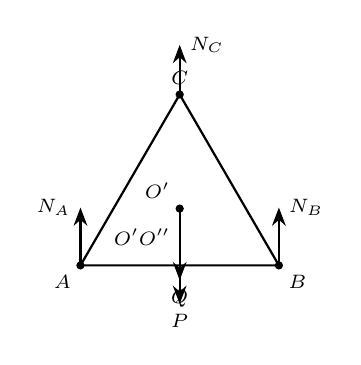
\begin{tikzpicture}[x=.7cm,y=.7cm,>=Stealth,font=\scriptsize]
  \coordinate (A) at (-1.8,-1.05); \coordinate (B) at (1.8,-1.05); \coordinate (C) at (0,2.05); \coordinate (Op) at (0,-.02);
  \draw[thick] (A)--(B)--(C)--cycle; \fill(A)circle(1.5pt)node[below left]{$A$}; \fill(B)circle(1.5pt)node[below right]{$B$}; \fill(C)circle(1.5pt)node[above]{$C$};
  \fill(Op)circle(1.5pt)node[above left]{$O'$}; \draw[dashed] (Op)--(0,-1.05) node[midway,left]{$O'O''$};
  \draw[->,thick] (Op)--+(0,-1.3) node[below]{$Q$}; \draw[->,thick] (0,-.75)--+(0,-1.0) node[below]{$P$};
  \draw[->,thick] (A)--+(0,1.05) node[left]{$N_A$}; \draw[->,thick] (B)--+(0,1.05) node[right]{$N_B$}; \draw[->,thick] (C)--+(0,.9) node[right]{$N_C$};
\end{tikzpicture}

\caption{第36届复赛第1题杯子偏移后的三脚几何与受力辅助图。}\label{fig:cpho36q01forces}
\end{figure}
\[
Q=(m+\lambda h_{\max})g,\qquad P=Mg,\qquad R'=R-r.
\]
杯子滑移后，几何关系和对称性给出
\[
O'A=O'B=\frac{a}{\sqrt3},\qquad
O'O''=\frac{a}{2\sqrt3},\qquad N_A=N_C.
\]
竖直方向和绕对称轴的平衡方程为
\[
N_A+N_B+N_C=Q+P,
\]
\[
Q R'+N_B\frac{a}{\sqrt3}-2N_A\frac{a}{2\sqrt3}=0.
\]
与滑移前的平均支持力 $(P+Q)/3$ 比较，得到
\[
\boxed{
\Delta N_B=-\frac{2\sqrt3}{3}\frac{R-r}{a}
\sqrt{1+\frac{4\pi\rho r^2H}{5m}}\,mg,
}
\]
\[
\boxed{
\Delta N_A=\Delta N_C=\frac{\sqrt3}{3}\frac{R-r}{a}
\sqrt{1+\frac{4\pi\rho r^2H}{5m}}\,mg.
}
\]
即靠近滑移方向对侧的凳脚 $B$ 支持力减小，另外两脚的支持力等量增加。

\subsection{转写依据}
题干、答案公式和题图分别依据 \texttt{CPHO36-Q01.md}、\texttt{CPHO36-Q01\_formula\_check\_v1.csv} 及题图核对入口。

% 题干转写：完成
% 解析转写：完成
% 图形核对：完成
\section{第36届复赛第2题：农用平板车碰撞与摩擦运动}
\subsection{题干}
农用平板车结构如图\ref{fig:cpho36q02}。两车轮半径均为 $r$、质量均为 $m$；平板长为 $l$、质量为 $2m$；两把手均为长 $2l$、质量 $m$ 的细杆。平板、把手和车轴固连，车轮可绕轴转动。（1）车轮被卡住而不能平移时，将水平把手由静止释放，求其与地面碰撞前的角速度。（2）在碰撞前撤去卡轮装置、碰撞时锁死车轮、碰后立即解锁；把手末端竖直方向不反弹，且把手和车轮与地面的滑动摩擦系数均为 $\mu$。求车轮开始运动至静止时车轴移动的距离。
\begin{figure}[htbp]\centering
\begin{tikzpicture}[scale=0.9,>=Stealth,font=\small]
  \draw[very thick] (-3.4,0.55) -- (2.55,0.55);
  \draw[very thick] (-3.4,-0.42) -- (2.55,-0.42);
  \draw[fill=gray!20,thick] (-0.25,-0.1) rectangle (2.55,0.55);
  \draw[thick] (0.15,0.05) circle (0.72);
  \draw[thick] (0.15,0.05) circle (0.10);
  \foreach \ang in {0,45,...,315} {\draw (0.15,0.05) -- ({0.15+0.65*cos(\ang)},{0.05+0.65*sin(\ang)});}
  \draw[fill=gray!25,thick] (0.15,0.05) circle (0.42);
  \draw[->] (0.15,0.05) -- (0.15,-0.67) node[midway,right] {$r$};
  \draw[<->] (-3.35,0.95) -- (1.15,0.95) node[midway,above] {$2l$};
  \draw[<->] (-0.25,-0.82) -- (2.55,-0.82) node[midway,below] {$l$};
  \node[left] at (-3.4,0.55) {把手末端};
  \node[right] at (2.55,0.55) {把手前端};
  \node[above] at (0.15,0.8) {$m$};
  \node[below] at (0.15,-0.92) {$m$};
  \node[above] at (1.45,0.55) {$2m$};
  \node[below] at (-2.0,0.55) {$m$};
  \node[below] at (-2.0,-0.42) {$m$};
  \draw[->,thick] (-3.9,-1.2) -- (3.2,-1.2) node[right] {$x$};
  \draw[fill] (0.15,0.05) circle (1.3pt) node[below right] {车轴};
\end{tikzpicture}

\caption{第36届复赛第2题农用平板车的 TikZ 结构重绘。}\label{fig:cpho36q02}
\end{figure}

\subsection{参考解答整理}
\paragraph{（1）把手落地前的角速度。} 把手、平板整体相对车轴的转动惯量和质心距分别为
\[
J=\frac43ml^2,\qquad r_C=\frac l4.
\]
质心下降高度为 $h=r/6$。由机械能守恒
\[
\frac12J\omega^2=4mgh,
\]
其中 $r_C$ 与 $h$ 的几何关系见图\ref{fig:cpho36q02geometry}。
\begin{figure}[htbp]\centering
\begin{tikzpicture}[x=.72cm,y=.72cm,>=Stealth,font=\scriptsize]
  \begin{scope}
    \draw[densely dashed] (-3,0)--(2.4,0);
    \draw[very thick] (-3,-1.46)--(2.2,.44);
    \fill (1,0) circle(1.4pt) node[above]{$O$};
    \fill (0,-.36) circle(1.4pt) node[below left]{$C$};
    \draw[->] (1,0)--(0,-.36) node[midway,below right]{$r_C$};
    \draw (1.55,0) arc(0:20:.55) node[midway,right]{$\theta$};
    \node at (-.15,-2) {(a) 质心位置};
  \end{scope}
  \begin{scope}[xshift=8.2cm]
    \draw[densely dashed] (-3,0)--(2.4,0);
    \draw[very thick] (-3,-1.46)--(2.2,.44);
    \fill (1,0) circle(1.4pt) node[above]{$O$};
    \fill (0,-.36) circle(1.4pt) node[below left]{$C$};
    \draw[->] (1,0)--(0,-.36) node[midway,below right]{$r_C$};
    \draw[<->] (-3,-1.46)--(-3,0) node[midway,left]{$r$};
    \draw[<->] (-3.12,-1.62)--(0,-.52) node[midway,below]{$3l/2$};
    \draw[<->] (-.32,-.36)--(-.32,0) node[midway,left]{$h$};
    \node at (-.15,-2) {(b) 质心下降};
  \end{scope}
\end{tikzpicture}

\caption{第36届复赛第2题把手--平板整体的质心位置与下降高度辅助图。}\label{fig:cpho36q02geometry}
\end{figure}
故
\[
\boxed{\omega=\sqrt{\frac{gr}{l}}.}
\]

\paragraph{（2）碰撞后的起动条件。} 碰前整体质心速率为
\[
v_{C1}=\omega r_C=\frac{\sqrt{grl}}4.
\]
令把手方向与速度分解所用夹角为 $\theta$，有
\[
\sin\theta=\frac{2r}{3l},\qquad
\cos\theta=\frac{\sqrt{9l^2-4r^2}}{3l}.
\]
由碰撞期间的动量定理，碰后系统水平初速度为
\[
v_0=\frac23(\sin\theta-\mu\cos\theta)v_{C1}
=\frac{\sqrt{gr}}6(\sin\theta-\mu\cos\theta).
\]
若
\[
\boxed{\mu\ge\tan\theta=\frac{2r}{\sqrt{9l^2-4r^2}},}
\]
则碰后不发生运动，$s=0$。

\paragraph{阶段I：又滑又滚。} 当 $\mu<\tan\theta$ 时，总滑动摩擦力为 $f=-6\mu mg$，整体质心加速度
\[
a_C=-\mu g.
\]
两车轮与把手--平板整体的受力关系见图\ref{fig:cpho36q02forces}上排。
由把手--平板与两车轮的受力、转动方程可得车轮角加速度
\[
\beta=\frac{8\mu g}{3r}.
\]
车轮达到纯滚动时的速度为
\[
v_1=\frac4{33}\sqrt{gr}(\sin\theta-\mu\cos\theta).
\]
该阶段车轴位移为
\[
s_1=\frac{57r}{78408\mu l^2}
\left(2r-\mu\sqrt{9l^2-4r^2}\right)^2.
\]

\paragraph{阶段II：纯滚动至停止。} 纯滚动阶段的质心加速度为
\[
a_{C2}=-\frac{\mu g}{11\mu\tan\theta+12}.
\]
静摩擦方向改变后的受力关系见图\ref{fig:cpho36q02forces}下排。
\begin{figure}[htbp]\centering
\begin{tikzpicture}[x=.58cm,y=.58cm,>=Stealth,font=\scriptsize]
  \begin{scope}
    \draw[thick] (-2.3,-1.55)--(2.3,-1.55);
    \draw[thick] (0,0) circle (1.25);
    \fill (0,0) circle(1.3pt) node[above right]{$O$};
    \draw[->,thick] (0,-1.25)--+(0,1.45) node[above]{$N_{01}$};
    \draw[->,thick] (0,0)--+(-1.45,0) node[left]{$N_{Ox}$};
    \draw[->,thick] (0,0)--+(0,-1.12) node[right]{$N_{Oy}$};
    \draw[->,thick] (-.72,-1.55)--+(-1.15,0) node[left]{$f_1$};
    \draw[->,thick] (0,0)--+(0,-1.9) node[below]{$2mg$};
    \draw[->,thick] (1.35,0)--+(1.05,0) node[right]{$a_C$};
    \draw[->] (.55,.95) arc(45:-55:.7) node[midway,right]{$\beta$};
    \node at (0,-2.6) {(c) 阶段I：两车轮};
  \end{scope}
  \begin{scope}[xshift=8.4cm]
    \draw[thick] (-3,-1.55)--(3,-1.55);
    \draw[very thick] (-2.8,-1.48)--(2.25,.45);
    \fill (.82,-.12) circle(1.4pt) node[above right]{$O$};
    \draw[densely dashed] (.82,-.12) circle (1.28);
    \fill (-.15,-.63) circle(1.3pt) node[above left]{$C$};
    \draw[->,thick] (-2.45,-1.55)--+(0,1.45) node[above]{$N$};
    \draw[->,thick] (-2.45,-1.55)--+(-1.05,0) node[left]{$\mu N$};
    \draw[->,thick] (.82,-.12)--+(1.2,0) node[right]{$N_{Ox}$};
    \draw[->,thick] (.82,-.12)--+(0,1.2) node[above]{$N_{Oy}$};
    \draw[->,thick] (-.15,-.63)--+(0,-1.15) node[below]{$4mg$};
    \draw (-1.6,-1.48) arc(0:20:.8) node[right]{$\theta$};
    \node at (0,-2.6) {(d) 阶段I：把手和平板};
  \end{scope}
\end{tikzpicture}

\vspace{.35cm}

\begin{tikzpicture}[x=.58cm,y=.58cm,>=Stealth,font=\scriptsize]
  \begin{scope}
    \draw[thick] (-2.3,-1.55)--(2.3,-1.55);
    \draw[thick] (0,0) circle (1.25);
    \fill (0,0) circle(1.3pt) node[above right]{$O$};
    \draw[->,thick] (0,-1.25)--+(0,1.45) node[above]{$N_{02}$};
    \draw[->,thick] (0,0)--+(-1.45,0) node[left]{$N_{Ox2}$};
    \draw[->,thick] (0,0)--+(0,-1.12) node[right]{$N_{Oy2}$};
    \draw[->,thick] (.72,-1.55)--+(1.15,0) node[right]{$f_2$};
    \draw[->,thick] (0,0)--+(0,-1.9) node[below]{$2mg$};
    \draw[->,thick] (1.35,0)--+(1.05,0) node[right]{$a_{C2}$};
    \draw[->] (.55,.95) arc(45:-55:.7) node[midway,right]{$\beta_2$};
    \node at (0,-2.6) {(e) 阶段II：两车轮};
  \end{scope}
  \begin{scope}[xshift=8.4cm]
    \draw[thick] (-3,-1.55)--(3,-1.55);
    \draw[very thick] (-2.8,-1.48)--(2.25,.45);
    \fill (.82,-.12) circle(1.4pt) node[above right]{$O$};
    \draw[densely dashed] (.82,-.12) circle (1.28);
    \fill (-.15,-.63) circle(1.3pt) node[above left]{$C$};
    \draw[->,thick] (-2.45,-1.55)--+(0,1.45) node[above]{$N_2$};
    \draw[->,thick] (-2.45,-1.55)--+(-1.05,0) node[left]{$\mu N_2$};
    \draw[->,thick] (.82,-.12)--+(1.2,0) node[right]{$N_{Ox2}$};
    \draw[->,thick] (.82,-.12)--+(0,1.2) node[above]{$N_{Oy2}$};
    \draw[->,thick] (-.15,-.63)--+(0,-1.15) node[below]{$4mg$};
    \draw (-1.6,-1.48) arc(0:20:.8) node[right]{$\theta$};
    \node at (0,-2.6) {(f) 阶段II：把手和平板};
  \end{scope}
\end{tikzpicture}

\caption{第36届复赛第2题两个运动阶段的车轮与把手--平板受力辅助图。}\label{fig:cpho36q02forces}
\end{figure}
由 $0-v_1^2=2a_{C2}s_2$，得
\[
s_2=\frac{16r}{9801\mu}
\left(2r-\mu\sqrt{9l^2-4r^2}\right)^2
\frac{11\mu r+6\sqrt{9l^2-4r^2}}{9l^2-4r^2}.
\]
因此在 $\mu<\tan\theta$ 时，车轴总位移为
\[
\boxed{s=s_1+s_2.}
\]

\subsection{转写依据}
题干、答案公式和题图分别依据 \texttt{CPHO36-Q02.md}、\texttt{CPHO36-Q02\_formula\_check\_v1.csv} 及题图核对入口。

% 题干转写：完成
% 解析转写：完成
% 图形核对：完成
\section{第36届复赛第3题：电磁轨道炮加速模型}
\subsection{题干}
如图\ref{fig:cpho36q03}，两根半径为 $b$、长度为 $L$、单位长度电阻为 $\lambda$ 的圆柱形平行导轨，所在对称面与水平面的夹角为 $\theta$。两导轨间的最近距离为 $d$（$d$ 很小）。质量为 $m$、直径为 $d$、电阻为 $R$ 的薄片状金属弹丸与导轨良好接触。导轨下端经同轴硬导线接入电流为 $I$ 的理想恒流源。忽略空气阻力、摩擦阻力和恒流源内部能量损耗，真空磁导率为 $\mu_0$。弹丸从导轨下端由静止开始加速，求：（1）弹丸所受磁场力；（2）出射速度；（3）加速过程中与出射时恒流源两端电压；（4）恒流源所做的功；（5）当 $\theta=0$ 且导轨、弹丸电阻均忽略时，出射动能与电源做功之比。
\begin{figure}[htbp]\centering
\begin{tikzpicture}[scale=0.9,>=Stealth,font=\small]
  % Coordinate u follows the rails; n is normal to the rail plane in the drawing.
  \begin{scope}[rotate=24]
    \draw[very thick,gray!70,line cap=round] (0,0.52) -- (7.3,0.52);
    \draw[very thick,gray!70,line cap=round] (0,-0.52) -- (7.3,-0.52);
    \foreach \x in {0,7.3} {
      \draw[fill=white,thick] (\x,0.52) ellipse (0.12 and 0.26);
      \draw[fill=white,thick] (\x,-0.52) ellipse (0.12 and 0.26);
    }
    \draw[fill=gray!45,thick] (3.55,-0.68) rectangle (3.86,0.68);
    \node[above] at (3.70,0.72) {弹丸};
    \draw[->,very thick] (3.70,0) -- (4.75,0) node[midway,above] {$F$};
    \draw[densely dashed] (0,1.00) -- (7.3,1.00);
    \draw[<->] (0,1.00) -- (7.3,1.00) node[midway,above] {$L$};
    \draw[<->] (5.75,-0.24) -- (5.75,0.24) node[midway,right] {$d$};
    \draw[<->] (6.95,0.52) -- (6.95,0.78) node[midway,right] {$b$};
    \node[above left] at (1.55,0.52) {导轨};
  \end{scope}
  \draw[thick] (-0.25,-0.62) -- (0.67,-0.62);
  \draw[thick] (-0.25,-0.62) -- (-0.25,0.15);
  \draw[thick] (0.67,-0.62) -- (0.67,-0.15);
  \draw[->,thick] (-0.25,-1.05) -- (0.67,-1.05);
  \draw[->,thick] (0.67,-1.05) -- (-0.25,-1.05);
  \node[below] at (0.21,-1.05) {恒流源 $I$};
  \draw[densely dashed] (0.55,-0.20) -- (5.25,-0.20);
  \draw (1.18,-0.20) arc[start angle=0,end angle=24,radius=0.63];
  \node at (1.48,0.03) {$\theta$};
\end{tikzpicture}

\caption{第36届复赛第3题电磁轨道炮简化模型的 TikZ 重绘。}\label{fig:cpho36q03}
\end{figure}

\subsection{参考解答整理}
\paragraph{（1）安培力。} 弹丸直径很小，可将两根载流导轨近似为半无限长直导线。弹丸上一点到一侧导轨轴线的距离为 $r'$ 时，磁感应强度为
\[
B=\frac{\mu_0 I}{4\pi r'}+\frac{\mu_0 I}{4\pi(d+2b-r')}.
\]
对弹丸横向积分（$b\le r'\le d+b$），得沿导轨向上的安培力
\[
\boxed{F=\frac{\mu_0 I^2}{2\pi}\ln\frac{d+b}{b}.}
\]

\paragraph{（2）出射速度。} 沿导轨列牛顿第二定律：
\[
F-mg\sin\theta=ma,
\qquad
a=\frac{\mu_0 I^2}{2\pi m}\ln\frac{d+b}{b}-g\sin\theta.
\]
弹丸做匀加速直线运动，因而
\[
\boxed{v_{\max}=\sqrt{2L\left(\frac{\mu_0 I^2}{2\pi m}\ln\frac{d+b}{b}-g\sin\theta\right)}.}
\]

\paragraph{（3）恒流源电压。} 设弹丸到导轨下端的距离为 $l$、速度为 $v=\mathrm{d}l/\mathrm{d}t$。回路中的磁通量和感应电动势为
\[
\Phi=\frac{\mu_0 I l}{\pi}\ln\frac{d+b}{b},
\qquad
\varepsilon=-\frac{\mu_0 Iv}{\pi}\ln\frac{d+b}{b}.
\]
由全电路欧姆定律 $U+\varepsilon=2\lambda lI+IR$，并代入 $v=at$、$l=at^2/2$，得到任意时刻的电压
\[
\boxed{U=\lambda Iat^2+IR+\frac{\mu_0 I}{\pi}\ln\frac{d+b}{b}\,at.}
\]
加速时间 $T=\sqrt{2L/a}$，故出射时
\[
\boxed{U_{\rm 出}=2\lambda IL+IR+\frac{\sqrt2\mu_0 I}{\pi}\ln\frac{d+b}{b}\sqrt{a}.}
\]

\paragraph{（4）电源做功。} 由 $W=\int_0^T UI\,\mathrm{d}t$，将三项分别积分，得到
\[
W=W_1+W_2+W_3,
\]
\[
W_1=\frac{2\sqrt2\lambda I^2}{3}L^{3/2}a^{-1/2},\qquad
W_2=I^2R\sqrt{2L}\,a^{-1/2},
\]
\[
\boxed{W_3=\frac{\mu_0 I^2L}{\pi}\ln\frac{d+b}{b}.}
\]
其中 $a$ 为第（2）问所得的加速度，故上式共同给出整个加速过程的电源做功。

\paragraph{（5）无电阻、水平导轨的极限。} 当 $\theta=0$ 且电阻可忽略时，
\[
E_{\max}=\frac{\mu_0 I^2L}{2\pi}\ln\frac{d+b}{b},
\qquad
W=\frac{\mu_0 I^2L}{\pi}\ln\frac{d+b}{b}.
\]
因此
\[
\boxed{\eta=\frac{E_{\max}}{W}=50\%.}
\]

\subsection{转写依据}
题干、答案公式与图形分别依据 \texttt{CPHO36-Q03.md}、\texttt{CPHO36-Q03\_formula\_check\_v1.csv} 和题图核对入口。评分分布为第（1）问8分、第（2）问6分、第（3）问14分、第（4）问6分、第（5）问6分。

% 题干转写：完成
% 解析转写：完成
% 图形核对：完成
\section{第36届复赛第4题：微孔竹板亥姆霍兹共振吸声}
\subsection{题干}
微孔竹板上的周期性长方形微孔可使孔中空气柱发生简谐振动；单个微孔及其后方空气层可简化为亥姆霍兹共振器，如图\ref{fig:cpho36q04}。微孔深度为 $l$，孔横截面积为 $S$，单孔后腔体体积为 $V_0$。声波传播视为绝热过程，满足 $v_s=\sqrt{\kappa/\rho}$，其中 $\kappa=-V\Delta p/\Delta V$。已知标准状态 $T=273\,\mathrm{K}$、$p=1.01\times10^5\,\mathrm{Pa}$，空气摩尔质量 $M_{\rm mol}=29.0\,\mathrm{g/mol}$、热容比 $\gamma=7/5$、气体常量 $R=8.31\,\mathrm{J/(K\cdot mol)}$。求：（1）标准状态下空气的密度和声速；（2）共振器吸收声波的频率；（3）吸收 $120\,\mathrm{Hz}$ 和 $200\,\mathrm{Hz}$ 时两种微孔面积之比。
\begin{figure}[htbp]\centering
\begin{tikzpicture}[scale=0.83,>=Stealth,font=\small]
  % The left panel preserves the periodic perforation feature without reproducing the source photograph.
  \draw[fill=brown!22,thick] (0,0) rectangle (3.15,2.45);
  \foreach \x in {0.22,0.48,...,2.92} {
    \foreach \y in {0.22,0.48,...,2.22} {
      \fill[black!65] (\x,\y) circle (0.026);
    }
  }
  \node[align=center,below] at (1.58,-0.10) {图a：周期性微孔竹板\\（结构示意）};

  % Cross section of the panel and its rear air layer.
  \begin{scope}[xshift=4.0cm]
    \draw[fill=gray!20,thick] (0,0) rectangle (5.4,0.30);
    \draw[fill=gray!12,thick] (0,0.30) rectangle (5.4,1.78);
    \foreach \x in {0.18,0.55,...,5.15} {
      \draw[fill=gray!60,draw=black] (\x,1.78) rectangle +(0.24,0.98);
    }
    \draw[thick] (0,2.76) -- (5.4,2.76) -- (5.4,0) -- (0,0) -- cycle;
    \draw[densely dashed] (1.82,0.05) -- (1.82,2.73);
    \draw[densely dashed] (2.34,0.05) -- (2.34,2.73);
    \draw[<->] (1.82,3.12) -- (2.34,3.12) node[midway,above] {$S$};
    \draw[<->] (5.78,1.78) -- (5.78,2.76) node[midway,right] {$l$};
    \node at (3.65,1.05) {空气层};
    \node[below] at (2.7,-0.10) {微孔板与后腔截面};

    % Corresponding lumped Helmholtz resonator.
    \begin{scope}[xshift=6.7cm]
      \draw[fill=gray!20,thick] (0,0) rectangle (1.62,1.42);
      \draw[fill=gray!55,thick] (0,0) rectangle (1.62,0.25);
      \draw[thick] (0.55,1.42) -- (0.55,2.38) -- (1.07,2.38) -- (1.07,1.42);
      \draw[<->] (1.32,1.42) -- (1.32,2.38) node[midway,right] {$l$};
      \draw[<->] (0.55,2.70) -- (1.07,2.70) node[midway,above] {$S$};
      \node at (0.81,0.80) {$V_0$};
      \node[below,align=center] at (0.81,-0.10) {亥姆霍兹\\共振器模型};
    \end{scope}
  \end{scope}
\end{tikzpicture}

\caption{第36届复赛第4题微孔竹板及亥姆霍兹共振器的 TikZ 重绘。}\label{fig:cpho36q04}
\end{figure}

\subsection{参考解答整理}
\paragraph{（1）标准状态下的密度与声速。} 理想气体状态方程为
\[
pV=\frac{M}{M_{\rm mol}}RT,
\qquad
\rho=\frac{M}{V}=\frac{M_{\rm mol}p}{RT}.
\]
故标准状态空气密度为
\[
\boxed{\rho_0=1.29\,\mathrm{kg/m^3}.}
\]
绝热过程满足 $pV^\gamma=\text{常量}$。微分后可得
\[
\kappa=-V\frac{\Delta p}{\Delta V}=\gamma p,
\qquad
v_s=\sqrt{\frac{\gamma p}{\rho}}.
\]
因此标准状态下
\[
\boxed{v_{s0}=\sqrt{\frac{(7/5)\times1.01\times10^5}{1.29}}=331\,\mathrm{m/s}.}
\]

\paragraph{（2）亥姆霍兹共振频率。} 微孔内空气柱质量为 $m=\rho Sl$。令空气柱向外位移为 $x$，则腔体体积改变量为 $\Delta V=Sx$，压强变化和回复力为
\[
\Delta p=-\frac{\gamma pSx}{V},
\qquad
F=S\Delta p=-\frac{\gamma pS^2}{V}x.
\]
由 $m\ddot{x}=F$ 得
\[
\ddot{x}=-\omega^2x,
\qquad
\omega=\sqrt{\frac{\gamma pS}{\rho lV}}.
\]
将 $V=V_0$ 与 $v_s=\sqrt{\gamma p/\rho}$ 代入，得到
\[
\boxed{f_0=\frac{v_s}{2\pi}\sqrt{\frac{S}{lV_0}}.}
\]

\paragraph{（3）两种孔面积之比。} 在 $l$、$V_0$ 和 $v_s$ 相同的条件下，$f\propto\sqrt S$，所以
\[
\frac{S_1}{S_2}=\left(\frac{f_{01}}{f_{02}}\right)^2
=\left(\frac{120}{200}\right)^2.
\]
故
\[
\boxed{\frac{S_1}{S_2}=0.36.}
\]

\subsection{转写依据}
题干、答案公式和图形分别依据 \texttt{CPHO36-Q04.md}、\texttt{CPHO36-Q04\_formula\_check\_v1.csv} 与题图核对入口。图a为照片型原图，成品以微孔周期结构示意替代，不嵌入原题截图。评分分布为第（1）问18分、第（2）问16分、第（3）问6分。

% 题干转写：完成
% 解析转写：完成
% 图形核对：完成
\section{第36届复赛第5题：阶跃型光纤耦合与全反射}
\subsection{题干}
阶跃型光纤内芯直径为 $50\,\mu\mathrm{m}$、折射率 $n_1=1.46$；玻璃外包层外径为 $125\,\mu\mathrm{m}$、折射率 $n_2=1.45$。现用直径 $D=3.00\,\mathrm{mm}$、折射率 $n=1.50$ 的微球透镜将氦氖激光器输出的圆柱形平行光束耦合入光纤，空气折射率 $n_0=1.00$，激光束轴、透镜球心和光纤轴重合，如图\ref{fig:cpho36q05}。求：（1）光纤端面的最大入射角；（2）平行光刚好会聚在光纤端面时，微球后表面顶点 $O$ 与端面的距离；（3）满足长距离传输条件的平行入射光束最大直径。
\begin{figure}[htbp]\centering
\begin{tikzpicture}[scale=0.91,>=Stealth,font=\small]
  \draw[densely dashed,gray] (-4.35,0) -- (4.75,0);
  \draw[->,very thick] (-4.4,1.08) -- (-2.65,1.08);
  \draw[->,very thick] (-4.4,-1.08) -- (-2.65,-1.08);
  \node[left] at (-4.4,0) {平行激光束};
  \draw[fill=cyan!10,thick] (-1.85,0) circle (1.72);
  \node[above] at (-1.85,1.88) {微球透镜};
  \node at (-1.85,-1.15) {$n=1.50$};
  \coordinate (A) at (-2.95,1.08);
  \coordinate (B) at (-2.95,-1.08);
  \coordinate (F) at (1.02,0);
  \draw[thick] (-4.4,1.08) -- (A) -- (F);
  \draw[thick] (-4.4,-1.08) -- (B) -- (F);
  \fill (F) circle (1.2pt) node[below] {$F$};
  \fill (-0.13,0) circle (1.2pt) node[below left] {$O$};
  \draw[thick] (1.55,-0.92) rectangle (4.55,0.92);
  \draw[fill=gray!20,thick] (1.55,-0.30) rectangle (4.55,0.30);
  \node at (3.05,0) {$n_1=1.46$};
  \node at (3.05,0.61) {$n_2=1.45$};
  \node at (3.05,-0.61) {$n_2=1.45$};
  \node[above] at (3.82,1.05) {光纤};
  \node[above] at (2.25,1.05) {芯径 $50\,\mu\mathrm{m}$};
  \draw[<->] (4.92,-0.92) -- (4.92,0.92) node[midway,right] {$125\,\mu\mathrm{m}$};
  \draw[<->] (-0.13,-1.92) -- (1.55,-1.92) node[midway,below] {$OF=0.75\,\mathrm{mm}$};
\end{tikzpicture}

\caption{第36届复赛第5题微球透镜耦合阶跃型光纤的 TikZ 重绘。}\label{fig:cpho36q05}
\end{figure}

\subsection{参考解答整理}
\paragraph{（1）端面最大入射角。} 设端面最大入射角为 $\theta$，进入纤芯后的折射角为 $\alpha$。由端面折射和芯--包层界面的全反射临界条件，
\[
n_0\sin\theta=n_1\sin\alpha,
\qquad
n_1\cos\alpha=n_2.
\]
相应的端面折射与芯--包层全反射临界光线见图\ref{fig:cpho36q05solution}左图。
消去 $\alpha$，得
\[
\sin\theta=\sqrt{\left(\frac{n_1}{n_0}\right)^2-\left(\frac{n_2}{n_0}\right)^2}
=\sqrt{1.46^2-1.45^2}\approx0.17.
\]
因此
\[
\boxed{\theta_{\max}=\arcsin(0.17)\approx9.8^\circ.}
\]

\paragraph{（2）微球后顶点到端面的距离。} 对微球前表面，平行光经球面折射后的一次像距为
\[
\frac{n_0}{o_1}+\frac{n}{i_1}=\frac{n-n_0}{r},
\qquad o_1=\infty,\quad r=\frac D2,
\]
故
\[
i_1=\frac{nD}{2(n-n_0)}=4.5\,\mathrm{mm}.
\]
相对于后表面顶点 $O$，该像为虚物，
\[
o_2=i_1-D=\frac{(n-2n_0)D}{2(n-n_0)}=-1.50\,\mathrm{mm},
\qquad r_2=-\frac D2.
\]
再对后表面应用球面折射公式，得到二次像距
\[
\boxed{i_2=\frac{(2n_0-n)D}{4(n-n_0)}=0.75\,\mathrm{mm}.}
\]
因此 $O$ 到光纤端面的距离为 $0.75\,\mathrm{mm}$。几何近轴解法同样给出 $OF=D/4=0.75\,\mathrm{mm}$。
\begin{figure}[htbp]\centering
\begin{tikzpicture}[x=.7cm,y=.7cm,>=Stealth,font=\scriptsize]
  \begin{scope}
    \draw[densely dashed] (-4,0)--(3.7,0);
    \draw[thick] (0,-1)--(3.1,-1)--(3.1,1)--(0,1)--cycle;
    \draw[thick] (0,.25)--(3.1,.25);
    \draw[thick] (0,-.25)--(3.1,-.25);
    \node at (1.55,.62) {$n_2$}; \node at (1.55,0) {$n_1$}; \node at (1.55,-.62) {$n_2$};
    \draw[->,thick] (-2.2,.75)--(0,.25);
    \draw[->,thick] (0,.25)--(1.1,-.25);
    \draw[->,thick] (1.1,-.25)--(2.65,.25);
    \draw (0,.04) arc(0:22:.42) node[right]{$\theta$};
    \draw (0.35,.24) arc(0:-24:.42) node[below right]{$\alpha$};
    \node[below] at (1.55,-1.2) {(a) 端面折射与全反射临界光线};
  \end{scope}
  \begin{scope}[xshift=10cm]
    \draw[densely dashed] (-4,0)--(5.2,0);
    \draw[thick] (0,0) circle (1.65);
    \coordinate (Oc) at (0,0);
    \fill (Oc) circle(1.3pt) node[below]{$O'$};
    \fill (1.65,0) circle(1.3pt) node[below]{$O$};
    \coordinate (A) at (-1.05,.95); \coordinate (B) at (1.42,.82); \coordinate (F) at (3.0,0); \coordinate (C) at (4.25,0);
    \fill (A) circle(1.3pt) node[above]{$A$}; \fill (B) circle(1.3pt) node[above]{$B$};
    \draw[->,thick] (-3.8,.95)--(A);
    \draw[thick] (A)--(B)--(F);
    \draw[dashed] (A)--(C); \draw[dashed] (B)--(C);
    \draw[dashed] (Oc)--(A) (Oc)--(B);
    \fill (F) circle(1.3pt) node[below]{$F$}; \fill (C) circle(1.3pt) node[below]{$C$};
    \node at (0,-1.05) {$n$};
    \draw (A) ++(-.32,0) arc(0:-35:.38) node[right]{$\alpha$};
    \draw (A) ++(.27,-.04) arc(-8:20:.44) node[above right]{$\gamma$};
    \draw (B) ++(.33,-.02) arc(-15:16:.4) node[right]{$\alpha$};
    \node[below] at (.55,-2) {(b) 微球折射的近轴几何};
  \end{scope}
\end{tikzpicture}

\caption{第36届复赛第5题端面临界光线与微球两次折射的几何辅助图。}\label{fig:cpho36q05solution}
\end{figure}

\paragraph{（3）可耦合的最大光束直径。} 微球的等效焦距为
\[
f_e=\frac{nD}{4(n-n_0)}=2.25\,\mathrm{mm}.
\]
当边缘光线在光纤端面的入射角恰为 $\theta_{\max}$ 时，利用近轴几何关系（忽略 $O[(d/D)^3]$ 项）有
\[
d_{\max}=\frac{nD\sin\theta_{\max}}{2(n-n_0)}.
\]
代入参数，
\[
\boxed{d_{\max}=0.76\,\mathrm{mm}.}
\]
故平行入射激光束的直径不能超过 $0.76\,\mathrm{mm}$。

\subsection{转写依据}
题干、答案公式和图形分别依据 \texttt{CPHO36-Q05.md}、\texttt{CPHO36-Q05\_formula\_check\_v1.csv} 与题图核对入口。评分分布为第（1）问8分、第（2）问20分、第（3）问12分。

% 题干转写：完成
% 解析转写：完成
% 图形核对：完成
\section{第36届复赛第6题：$\pi$介子衰变与$\mu$子相对论寿命}
\subsection{题干}
高速 $\pi$ 介子发生衰变
\[
\pi\rightarrow\mu+\bar\nu_\mu.
\]
已知 $m_\pi=139.57061\,\mathrm{MeV}/c^2$、$m_\mu=105.65837\,\mathrm{MeV}/c^2$，反中微子静止质量可忽略。实验室系中 $\pi$ 介子速度为 $v=0.965c$，其中 $c=3.00\times10^8\,\mathrm{m/s}$。求：（1）衰变产生的 $\mu$ 子最大和最小速率；（2）$\mu$ 子从距地面 $h=10000\,\mathrm{m}$ 高空竖直下落时，若静止 $\mu$ 子半衰期 $T_{1/2}^{(0)}=1.523\,\mu\mathrm{s}$，地面观察者观测到 $\mu$ 子的最大概率。

\subsection{参考解答整理}
\paragraph{（1）$\pi$介子静止系中的$\mu$子速度。} 在相对于 $\pi$ 介子静止的 $S'$ 系中，动量和能量守恒分别为
\[
\boldsymbol p'_\mu+\boldsymbol p'_{\bar\nu}=0,
\qquad
E'_\mu+E'_{\bar\nu}=m_\pi c^2.
\]
反中微子质量近似为零，联立相对论能量--动量关系可得
\[
\boxed{u'_\mu=\frac{m_\pi^2-m_\mu^2}{m_\pi^2+m_\mu^2}c=0.2714c.}
\]

\paragraph{（2）实验室系中的速度极值。} $\mu$ 子相对 $\pi$ 介子运动方向与母粒子飞行方向平行、反平行时，实验室系速率分别取最大、最小值。由一维相对论速度变换，
\[
u_{\mu,\max}=\frac{u'_\mu+v}{1+u'_\mu v/c^2},
\qquad
u_{\mu,\min}=\frac{-u'_\mu+v}{1-u'_\mu v/c^2}.
\]
代入 $u'_\mu=0.2714c$、$v=0.965c$，得到
\[
\boxed{u_{\mu,\max}=0.980c=2.94\times10^8\,\mathrm{m/s},}
\]
\[
\boxed{u_{\mu,\min}=0.940c=2.82\times10^8\,\mathrm{m/s}.}
\]

\paragraph{（3）地面处的最大存活概率。} 最大速率对应最短飞行时间：
\[
(\Delta t)_{\min}=\frac{h}{u_{\mu,\max}}
=\frac{10000}{0.980\times3.00\times10^8}
=3.40\times10^{-5}\,\mathrm{s}.
\]
由时间膨胀，地面系中半衰期为
\[
T_{1/2}=\frac{T_{1/2}^{(0)}}{\sqrt{1-u_{\mu,\max}^2/c^2}}
=0.765\times10^{-5}\,\mathrm{s}.
\]
使用半衰期形式的衰变律 $P=2^{-\Delta t/T_{1/2}}$，得
\[
\boxed{P_{\max}=2^{-(\Delta t)_{\min}/T_{1/2}}=0.0459\approx4.59\%.}
\]
等价地，取静止平均寿命 $\tau_0=T_{1/2}^{(0)}/\ln2=2.197\,\mu\mathrm{s}$，经时间膨胀后代入 $P=\exp(-\Delta t/\tau)$，得到同一量级的 $4.55\%$ 至 $4.59\%$ 结果。

\subsection{转写依据}
题干与答案公式分别依据 \texttt{CPHO36-Q06.md} 和 \texttt{CPHO36-Q06\_formula\_check\_v1.csv}。原题无题图，故本题不添加TikZ图件。评分分布为第（1）问26分、第（2）问14分。

% 题干转写：完成
% 解析转写：完成
% 图形核对：完成
\section{第36届复赛第7题：闪电、电离层光环与球形闪电模型}
\subsection{题干}
雷电云中上部带正电、下部带负电，云地闪电把云底负电荷释放到地面，如图\ref{fig:cpho36q07cloud}。题目依次给定圆柱形雷电云的均匀电场 $E=0.15\,\mathrm{MV/m}$、半径 $r=2.5\,\mathrm{km}$、高度 $d=1.0\,\mathrm{km}$；负电荷层距地 $h=6.0\,\mathrm{km}$；闪电通道总电荷 $2.5\,\mathrm C$ 和空气击穿阈值 $3.0\,\mathrm{MV/m}$；电离层底面高度约 $80\,\mathrm{km}$、光环半径 $100\,\mathrm{km}$；以及在 $12\,\mathrm{km}$ 高空悬浮 $50\,\mathrm{kg}$ 载荷的氦气球参数。求雷电云的电势差、电荷和能量，地表电场，闪电通道直径及电荷密度分布，电离层光环扩展速度和气球体积。
\begin{figure}[htbp]\centering
\begin{tikzpicture}[scale=0.86,>=Stealth,font=\small]
  \draw[thick] (-3.35,-2.15) -- (3.35,-2.15);
  \foreach \x in {-3.1,-2.7,...,3.1} {\draw (\x,-2.15) -- +(0.20,-0.16);}
  \node[below] at (0,-2.25) {地面};
  \node[cloud,cloud puffs=13,cloud puff arc=105,aspect=2.2,draw,fill=gray!10,minimum width=5.2cm,minimum height=2.2cm] (cloud) at (0,0.72) {};
  \foreach \x/\y in {-1.4/1.08,-0.8/1.32,-0.2/1.10,0.4/1.36,1.05/1.10} {\node at (\x,\y) {+};}
  \foreach \x/\y in {-1.25/0.25,-0.65/0.05,0.05/0.24,0.72/0.02,1.32/0.28} {\node at (\x,\y) {$-$};}
  \draw[very thick] (-0.75,0.70) -- (-0.48,0.36) -- (-0.72,0.36) -- (-0.42,-0.08);
  \draw[very thick] (0.90,0.84) -- (1.17,0.48) -- (0.94,0.48) -- (1.22,0.07);
  \draw[very thick] (0.10,0.10) -- (-0.08,-0.35) -- (0.14,-0.35) -- (-0.12,-1.42);
  \node[right] at (0.18,-0.76) {云地闪电};
  \draw[<->] (-3.0,-2.0) -- (-3.0,1.92) node[midway,left] {$12\,\mathrm{km}$};
  \draw[<->] (-2.52,-2.0) -- (-2.52,-0.15) node[midway,left] {$6\,\mathrm{km}$};
  \node[above] at (0,1.92) {雷电云电荷分布};
\end{tikzpicture}

\caption{第36届复赛第7题雷电云电荷分布的 TikZ 重绘。}\label{fig:cpho36q07cloud}
\end{figure}

\subsection{参考解答整理}
\paragraph{（1）圆柱雷电云的电学量。} 将带电区域近似为平行板电容器，面积 $S=\pi r^2$，有
\[
C=\frac{\varepsilon_0S}{d},\qquad U=Ed=150\,\mathrm{MV}.
\]
从而
\[
\boxed{Q=CU=26\,\mathrm C,\qquad W=\frac12QU=2.0\times10^9\,\mathrm J.}
\]

\paragraph{（2）云正下方的地表电场。} 把地面看作平面导体，采用镜像法并先以点电荷近似，有
\[
E=\frac{Q}{2\pi\varepsilon_0}\left[\frac1{(h+d)^2}-\frac1{h^2}\right]
\approx-3.5\,\mathrm{kV/m}.
\]
负号表示场方向垂直地面向上。将两电荷层按有限带电圆盘积分，可得到更精确的估算
\[
\boxed{E_{\rm 地面}\approx-2.8\,\mathrm{kV/m}.}
\]

\paragraph{（3）闪电通道尺度与径向电荷密度。} 通道长度取 $h=6.0\,\mathrm{km}$ 时，线电荷密度
\[
\eta=\frac Qh=4.2\times10^{-4}\,\mathrm{C/m}.
\]
通道外电场 $E(r')=\eta/(2\pi\varepsilon_0r')$。令柱面场达到击穿阈值，得通道直径
\[
\boxed{D\approx\frac{\eta}{\pi\varepsilon_0E_{\rm 击穿}}=5.0\,\mathrm m.}
\]
对通道内同轴高斯柱面应用高斯定律，并忽略中心放电细路径的尺度，
\[
r\varepsilon_0E_{\rm 击穿}=\int_0^r r'\rho(r')\,\mathrm dr',
\]
故
\[
\boxed{\rho(r)=\frac{\varepsilon_0E_{\rm 击穿}}{r}.}
\]

\paragraph{（4）电离层底部光环。} 无线电波自近地闪电点 $O$ 以球面波传播；波前掠过而不能进入电离层底面，交线形成向外扩展的光环，如图\ref{fig:cpho36q07ring}。设 $OA=80\,\mathrm{km}$、$AB=r$，则
\[
\cos\theta=\frac{AB}{OB}=\frac{AB}{\sqrt{OA^2+AB^2}},
\qquad
v_{\rm 环}=\frac{c}{\cos\theta}
=c\frac{\sqrt{OA^2+AB^2}}{AB}.
\]
当 $AB=100\,\mathrm{km}$ 时，
\[
\boxed{v_{\rm 环}=1.28c=3.8\times10^8\,\mathrm{m/s}.}
\]
这是球面波与电离层平面的交线所呈现的几何扩展速度，并非物质或信息以超光速传播。
\begin{figure}[htbp]\centering
\begin{tikzpicture}[scale=0.86,>=Stealth,font=\small]
  \draw[thick] (-3.55,0) -- (3.55,0);
  \foreach \x in {-3.3,-2.9,...,3.3} {\draw (\x,0) -- +(0.18,-0.13);}
  \node[below] at (-2.9,-0.16) {地面};
  \draw[very thick] (-3.55,2.10) -- (3.55,2.10);
  \node[above right] at (-3.45,2.10) {电离层底面};
  \coordinate (O) at (0,0);
  \fill (O) circle (1.3pt) node[below left] {$O$};
  \draw[thick] (2.10,0) arc[start angle=0,end angle=180,radius=2.10];
  \draw[thick] (2.90,0) arc[start angle=0,end angle=180,radius=2.90];
  \draw[densely dotted,thick] (3.45,0) arc[start angle=0,end angle=180,radius=3.45];
  \coordinate (A) at (0,2.10);
  \coordinate (B) at ({sqrt(2.90*2.90-2.10*2.10)},2.10);
  \coordinate (D) at ({sqrt(3.45*3.45-2.10*2.10)},2.10);
  \coordinate (C) at ({sqrt(3.45*3.45-2.10*2.10)+0.38},2.10);
  \fill (A) circle (1.1pt) node[above right] {$A$};
  \fill (B) circle (1.1pt) node[above] {$B$};
  \fill (D) circle (1.1pt) node[above] {$D$};
  \draw[thick] (O) -- (B);
  \draw[thick] (B) -- (C);
  \node[below] at (1.00,2.10) {$AB=r$};
  \draw (B) ++(-0.26,0) arc[start angle=180,end angle=226,radius=0.26];
  \node at (2.17,1.62) {$\theta$};
  \node[below right] at (C) {$C$};
  \node[left] at (-3.5,1.05) {$OA=80\,\mathrm{km}$};
\end{tikzpicture}

\caption{电离层底部光环产生与扩展过程的 TikZ 示意图。}\label{fig:cpho36q07ring}
\end{figure}

\paragraph{（5）$12\,\mathrm{km}$高空气球体积。} 悬浮条件为
\[
m_{\rm 载荷}g+\rho_{\rm He}Vg=\rho_1Vg,
\qquad V=\frac{m_{\rm 载荷}}{\rho_1-\rho_{\rm He}}.
\]
温度递减关系 $T=T_0-az$（$a=5.0\times10^{-3}\,\mathrm{K/m}$）与静力平衡、理想气体状态方程共同给出
\[
p=p_0\left(1-\frac{az}{T_0}\right)^{Mg/(aR)},
\qquad
\rho=\rho_0\left(1-\frac{az}{T_0}\right)^{Mg/(aR)-1}.
\]
在 $z=12\,\mathrm{km}$ 处取 $\rho_1\approx0.31\,\mathrm{kg/m^3}$，代入 $m_{\rm 载荷}=50\,\mathrm{kg}$、$\rho_{\rm He}=0.18\,\mathrm{kg/m^3}$，得到
\[
\boxed{V\approx3.8\times10^2\,\mathrm{m^3}.}
\]

\subsection{转写依据}
题干、答案公式与图形分别依据 \texttt{CPHO36-Q07.md}、\texttt{CPHO36-Q07\_formula\_check\_v1.csv}、题图核对入口和第（4）问解题图页面。评分分布为第（1）问8分、第（2）问10分、第（3）问18分、第（4）问16分、第（5）问18分。

% 题干转写：完成
% 解析转写：完成
% 图形核对：完成
\section{第37届复赛第1题：高铁空气弹簧劲度系数模型}
\subsection{题干}
高铁空气弹簧由主气室、附加气室及阀门组成，如图\ref{fig:cpho37q01}。平衡时主气室压强、体积分别为 $p_{10}$、$V_{10}$，附加气室容积为 $V_2$，大气压强为 $p_0$。主气室对簧上负载的竖直作用力为 $F=(p_1-p_0)A_e$。在小振幅条件下，主气室体积和有效承载面积随负载相对平衡位置的向下位移 $y$ 线性变化：
\[
\frac{\mathrm dV_1}{\mathrm dy}=-\alpha,\qquad
\frac{\mathrm dA_e}{\mathrm dy}=\beta,\qquad \alpha,\beta>0.
\]
求阀门关闭、阀门打开时，分别在等温与绝热条件下空气弹簧劲度系数 $K=\mathrm dF/\mathrm dy$ 与 $A_e$ 的关系。
\begin{figure}[htbp]\centering
\begin{tikzpicture}[scale=0.95,>=Stealth,font=\small]
  \draw[fill=gray!15,thick] (0.7,2.55) rectangle (3.85,3.45);
  \node at (2.28,3.00) {簧上负载};
  \draw[fill=gray!25,thick] (2.05,2.12) rectangle (2.55,2.55);
  \draw[fill=white,thick,rounded corners=8pt] (1.35,0.55) rectangle (3.25,2.12);
  \draw[fill=gray!25,thick] (1.18,0.26) rectangle (3.42,0.55);
  \node at (2.30,1.33) {主气室};
  \draw[fill=white,thick,rounded corners=8pt] (-2.55,0.50) rectangle (-0.78,1.88);
  \draw[fill=gray!25,thick] (-2.70,0.22) rectangle (-0.63,0.50);
  \node at (-1.67,1.17) {附加气室};
  \draw[very thick] (-1.67,1.88) .. controls (-1.50,2.48) and (0.25,2.40) .. (1.35,1.92);
  \draw[fill=white,thick] (-2.10,2.14) rectangle (-1.50,2.36);
  \draw[thick] (-1.80,2.36) -- (-1.80,2.62);
  \node[left] at (-1.90,2.55) {阀门};
  \draw[thick] (-3.1,0.18) -- (3.85,0.18);
  \foreach \x in {-2.95,-2.55,...,3.65} {\draw (\x,0.18) -- +(0.18,-0.12);}
  \draw[<->] (3.78,0.55) -- (3.78,2.12) node[midway,right] {$y$（向下为正）};
\end{tikzpicture}

\caption{第37届复赛第1题高铁空气弹簧结构的 TikZ 重绘。}\label{fig:cpho37q01}
\end{figure}

\subsection{参考解答整理}
\paragraph{统一推导。} 用多方过程方程
\[
p_1V_1^n=\text{常量}
\]
统一处理两种热力学过程。由 $F=(p_1-p_0)A_e$，有
\[
K=(p_1-p_0)\frac{\mathrm dA_e}{\mathrm dy}
+\frac{\mathrm dp_1}{\mathrm dy}A_e.
\]
对过程方程微分，并代入 $\mathrm dV_1/\mathrm dy=-\alpha$、$\mathrm dA_e/\mathrm dy=\beta$，阀门关闭时得到通式
\[
K=\frac{\alpha n p_{10}V_{10}^n}{V_1^{n+1}}A_e
+\beta\left[p_{10}\left(\frac{V_{10}}{V_1}\right)^n-p_0\right].
\]

\paragraph{（1）阀门关闭。} 上下乘客变化缓慢时，气体近似等温，$n=1$：
\[
\boxed{K=\frac{\alpha p_{10}V_{10}}{V_1^2}A_e
+\beta\left(\frac{p_{10}V_{10}}{V_1}-p_0\right).}
\]
剧烈振动时可近似绝热。由 $C_V=\frac52R$，
\[
\gamma=\frac{C_P}{C_V}=\frac{C_V+R}{C_V}=\frac75.
\]
于是
\[
\boxed{K=\frac{7\alpha p_{10}V_{10}^{7/5}}{5V_1^{12/5}}A_e
+\beta\left[p_{10}\left(\frac{V_{10}}{V_1}\right)^{7/5}-p_0\right].}
\]

\paragraph{（2）阀门打开。} 低频、缓慢变形时，主气室与附加气室压强相同，二者作为整体作等温变化：
\[
\boxed{K=\frac{\alpha p_{10}(V_{10}+V_2)}{(V_1+V_2)^2}A_e
+\beta\left[\frac{p_{10}(V_{10}+V_2)}{V_1+V_2}-p_0\right].}
\]
高频、快速变形时，来不及通过连通管流动的气体仅限于主气室，因此仍为主气室的绝热结果：
\[
\boxed{K=\frac{7\alpha p_{10}V_{10}^{7/5}}{5V_1^{12/5}}A_e
+\beta\left[p_{10}\left(\frac{V_{10}}{V_1}\right)^{7/5}-p_0\right].}
\]

\subsection{转写依据}
题干、答案公式和图形分别依据 \texttt{CPHO37-Q01.md}、\texttt{CPHO37-Q01\_formula\_check\_v1.csv} 与题图核对入口。评分分布为第（1）问32分、第（2）问8分。

% 题干转写：完成
% 解析转写：完成
% 图形核对：完成
\section{第40届复赛第1题：手机镜头的主点与等效焦距}

\subsection{题干}

智能手机镜头可视为结构固定的共轴理想透镜组。其物像关系等效于凸透镜的物像关系，但应以物方主点 $H$ 和像方主点 $H'$ 作为物距、像距和焦距的参考点，如图\ref{fig:cpho40q01}所示；本题所有光路均满足近轴条件。

\begin{figure}[htbp]
  \centering
  \begin{tikzpicture}[>=Stealth,scale=0.9]
  \draw[->] (-5.0,0) -- (-0.2,0);
  \draw[dashed,thick] (-3.35,-0.85) rectangle (-1.35,0.85);
  \node[below] at (-2.35,-0.85) {透镜组};
  \fill (-4.55,0) circle (1.5pt) node[above] {物};
  \fill (-2.85,0) circle (1.5pt) node[below] {$H$};
  \fill (-1.83,0) circle (1.5pt) node[below] {$H'$};
  \fill (-0.62,0) circle (1.5pt) node[above] {像};
  \draw[<->] (-4.55,-0.34) -- (-2.85,-0.34) node[midway,below] {物距};
  \draw[<->] (-1.83,-0.34) -- (-0.62,-0.34) node[midway,below] {像距};
  \draw[->] (1.2,0) -- (5.8,0);
  \draw[thick] (3.50,-1.0) -- (3.50,1.0);
  \draw[<->] (3.26,0.77) -- (3.74,0.77);
  \fill (1.60,0) circle (1.5pt) node[above] {物};
  \fill (5.25,0) circle (1.5pt) node[above] {像};
  \node[below] at (3.50,-1.0) {薄透镜};
  \draw[<->] (1.60,-0.34) -- (3.50,-0.34) node[midway,below] {物距};
  \draw[<->] (3.50,-0.34) -- (5.25,-0.34) node[midway,below] {像距};
\end{tikzpicture}

  \caption{第40届复赛第1题图1a的TikZ重绘：透镜组与薄透镜的物像关系。}
  \label{fig:cpho40q01}
\end{figure}

\begin{enumerate}
  \item 长度为 $l$ 的刻度尺垂直于光轴，在物距为 $u_1$ 和 $u_2$ 的位置分别成像。测得刻度尺移动距离 $s=u_2-u_1$，对应像长为 $l_1$、$l_2$。求镜头的等效焦距 $F$ 和物距 $u_1$。
  \item 透镜组由焦距为 $f_1$、$f_2$ 的两块共轴薄凸透镜组成，光心为 $O_1$、$O_2$，间距为 $d$。透镜组存在横向放大率为 $+1$ 的一对主平面，主点为 $H$、$H'$。求 $H$ 相对 $O_1$ 的物距、$H'$ 相对 $O_2$ 的像距，以及物方、像方焦距 $F$、$F'$。
\end{enumerate}

\subsection{参考解答整理}

\paragraph{（1）（i）利用两次成像测量等效焦距。}
对物距 $u_1$、像距 $v_1$，薄透镜成像关系与横向放大关系为
\[
\frac1{u_1}+\frac1{v_1}=\frac1F,
\qquad \frac{v_1}{u_1}=\frac{l_1}{l}.
\]
故
\[
u_1=F\left(1+\frac{l}{l_1}\right),
\qquad
u_2=F\left(1+\frac{l}{l_2}\right).
\]
由 $s=u_2-u_1$ 得
\[
F=\frac{s}{\frac{l}{l_2}-\frac{l}{l_1}}
=\frac{sl_1l_2}{l(l_1-l_2)}.
\]

\paragraph{（1）（ii）确定物距 $u_1$。}
将等效焦距代回 $u_1=F(1+l/l_1)$，得到
\[
\boxed{u_1=\frac{sl_2(l_1+l)}{l(l_1-l_2)}}.
\]

\paragraph{（2）（i）两薄透镜组成的主点。}
设透镜1、2的物距和像距分别为 $u_1,v_1$ 和 $u_2,v_2$。有
\[
\frac1{u_1}+\frac1{v_1}=\frac1{f_1},
\qquad
\frac1{u_2}+\frac1{v_2}=\frac1{f_2},
\]
\[
m_1=-\frac{v_1}{u_1},\qquad m_2=-\frac{v_2}{u_2},
\qquad u_2=d-v_1=d-\frac{u_1f_1}{u_1-f_1}.
\]
主平面定义要求 $m=m_1m_2=+1$。代入后得到物方主点 $H$ 相对 $O_1$ 的物距和像方主点 $H'$ 相对 $O_2$ 的像距：
\[
u_H=\frac{f_1d}{d-f_1-f_2},
\qquad
v_{H'}=\frac{f_2d}{d-f_1-f_2}.
\]
\paragraph{（2）（ii）物方焦距与像方焦距。}
当物距趋于无穷大时，第一块透镜的像距为 $f_1$，从而
\[
v_{F'}=\frac{(d-f_1)f_2}{d-f_1-f_2}.
\]
于是像方焦距和物方焦距为
\[
F'=v_{F'}-v_{H'}=-\frac{f_1f_2}{d-f_1-f_2},
\qquad
F=F',
\]
等价地，
\[
\frac1F=\frac1{F'}=\frac1{f_1}+\frac1{f_2}-\frac{d}{f_1f_2}.
\]

% 题干转写：完成
% 解析转写：完成
% 图形核对：完成
\section{第40届复赛第2题：半圆管中活塞的稳定性与临界温度}

\subsection{题干}

如图\ref{fig:cpho40q02}，将一根粗细均匀、两端封闭的细玻璃管弯成半径为 $r$ 的半圆环，竖直固定在水平地面上；玻璃管横截面半径远小于 $r$。管中有质量为 $m$ 的薄金属活塞，活塞与管壁密接而摩擦可忽略。活塞相对竖直方向的角位置记为 $\theta$。活塞两侧各有 $n$ 摩尔理想气体，气体温度始终等于外界绝对温度 $T$，所有状态变化均为准静态过程。已知重力加速度为 $g$、普适气体常量为 $R$。

\begin{figure}[htbp]
  \centering
  \begin{tikzpicture}[>=Stealth,scale=0.92]
  \draw[thick] (-3.2,0) -- (3.2,0);
  \foreach \x in {-3.1,-2.8,...,3.1} {\draw[gray] (\x,0) -- +(0.22,-0.16);}
  \draw[very thick] (-2.55,0) arc[start angle=180,end angle=0,radius=2.55];
  \draw[very thick] (-2.18,0) arc[start angle=180,end angle=0,radius=2.18];
  \coordinate (O) at (0,0);
  \coordinate (P) at (-1.05,1.91);
  \draw[thick] ($(P)+(-0.18,-0.12)$) -- ($(P)+(0.18,0.12)$);
  \fill (O) circle (1.5pt) node[below right] {$O$};
  \draw[densely dashed] (O) -- (0,2.55);
  \draw[densely dashed] (O) -- (P);
  \draw[<->] (0.18,0.1) -- (0.18,2.45) node[midway,right] {$r$};
  \draw[->] (0,0.72) arc[start angle=90,end angle=119,radius=0.72];
  \node at (-0.28,0.92) {$\theta$};
  \node[below] at (0,-0.26) {水平地面};
\end{tikzpicture}

  \caption{第40届复赛第2题图2a的TikZ重绘：半圆玻璃管、活塞与角位置。}
  \label{fig:cpho40q02}
\end{figure}

\begin{enumerate}
  \item 当 $T$ 高于临界温度 $T_c$ 时，玻璃管正中央 $\theta=0$ 是活塞的稳定平衡位置。求 $T_c$，并求此处小振动的圆频率。
  \item 当 $T=T_c$ 时，判断 $\theta=0$ 处平衡的稳定性。
  \item 当 $T<T_c$ 时，求稳定平衡位置 $\theta_0$ 所满足的方程，并给出 $T$ 略低于 $T_c$ 时 $\theta_0$ 的最低阶近似。
  \item 当 $T<T_c$ 时，求稳定平衡位置附近圆频率 $\omega_0(\theta_0)$；再给出 $T$ 略高于和略低于 $T_c$ 时圆频率随温度的关系。
  \item 当 $T<T_c$ 时，若活塞初速度近似为零，求其由正中央到达角位置 $\theta$ 时的角速度大小。
\end{enumerate}

\subsection{参考解答整理}

\paragraph{（1）临界温度与中央位置的小振动。}
活塞偏离中央一个小角度时，沿管切线方向的运动方程为
\[
mr\ddot\theta=mg\sin\theta-
\frac{nRT}{r(\pi/2-\theta)}+
\frac{nRT}{r(\pi/2+\theta)}.
\]
在线性近似下，
\[
\ddot\theta=\frac1r\left(g-\frac{8nRT}{\pi^2rm}\right)\theta.
\]
中央位置稳定要求括号内为负，因此
\[
T_c=\frac{\pi^2mgr}{8nR}.
\]
当 $T>T_c$ 时，活塞在中央位置作简谐振动，圆频率为
\[
\omega=\sqrt{\frac1r\left(\frac{8nRT}{\pi^2rm}-g\right)}
=\sqrt{\frac gr\frac{T-T_c}{T_c}}.
\]

\paragraph{（2）临界点的稳定性。}
令 $T=T_c$，保留最低非零项，得到
\[
\ddot\theta=-\frac{(24+\pi^2)g}{6\pi^2r}\theta^3.
\]
加速度方向与 $\theta$ 的符号相反，故中央位置仍为稳定平衡位置；其回复作用为三阶小量，而非线性回复力。

\paragraph{（3）低温下的对称破缺平衡位置。}
对非零平衡位置 $\theta_0$，合力为零给出
\[
mg\sin\theta_0-
\frac{nRT}{r(\pi/2-\theta_0)}+
\frac{nRT}{r(\pi/2+\theta_0)}=0.
\]
利用 $T_c$ 可整理为
\[
\frac{T}{T_c}=
\left(1-\frac{4\theta_0^2}{\pi^2}\right)
\frac{\sin\theta_0}{\theta_0}.
\]
当 $T$ 略低于 $T_c$ 时，
\[
\theta_0=\pm\sqrt{
\frac{6\pi^2}{24+\pi^2}\frac{T_c-T}{T_c}}
\]
，正、负号分别对应竖直线左右两侧的稳定位置。

\paragraph{（4）低温平衡位置附近的振动。}
在 $\theta_0$ 附近写 $\theta_0+\theta$，其中 $\theta$ 为微小扰动。线性化后得到
\[
\omega_0=
\sqrt{\frac{g\cos\theta_0}{r}
\left[
\frac{\tan\theta_0}{\theta_0}
\frac{\pi^2/2+2\theta_0^2}{\pi^2/2-2\theta_0^2}-1
\right]}.
\]
当 $T$ 略低于 $T_c$ 时，$|\theta_0|\ll1$，从而
\[
\omega_0\approx\sqrt{\frac{2g}{r}\frac{T_c-T}{T_c}}.
\]
这与 $T$ 略高于 $T_c$ 时的结果共同刻画了临界温度两侧的频率变化。

\paragraph{（5）由能量积分求角速度。}
将运动方程两边乘以 $d\theta$，并使用初始角速度近似为零的条件，有
\[
\frac12mr^2\dot\theta^2
=mg(1-\cos\theta)+\frac{nRT}{r}
\ln\left(1-\frac{4\theta^2}{\pi^2}\right).
\]
故活塞到达可及角位置 $\theta$ 时的角速度大小为
\[
|\dot\theta|=
\sqrt{\frac{2g}{r}(1-\cos\theta)+
\frac{2nRT}{mr^2}\ln\left(1-\frac{4\theta^2}{\pi^2}\right)}.
\]

\subsection{转写依据}

题干依据第40届复赛第2题题面视觉转写稿，解析依据答案页公式核对表；图形依据图2a重裁候选图的结构和标注重绘。对应文件为\texttt{CPHO40-Q02\_transcription\_v1.md}、\texttt{CPHO40-Q02\_formula\_check\_v1.csv}与\texttt{CPHO40-Q02\_figure\_check\_v1.csv}。

% 题干转写：完成
% 解析转写：完成
% 图形核对：完成
\section{第40届复赛第3题：楔块上匀质圆球的滚动与滑动}

\subsection{题干}

如图\ref{fig:cpho40q03}，倾角为 $\theta$、质量为 $M$ 的三角形楔块放在光滑的水平地面上。其斜面上有一个质量为 $m$、半径为 $r$ 的匀质圆球；圆球从静止开始自由向下运动，整个过程中楔块不发生转动。重力加速度大小为 $g$。设圆球与楔块间的静摩擦因数和滑动摩擦因数均为 $\mu$。

\begin{figure}[htbp]
  \centering
  \begin{tikzpicture}[>=Stealth,scale=0.9]
  \draw[thick] (-4.0,-1.5) -- (4.0,-1.5);
  \fill[gray!15] (-2.9,-1.5) -- (2.7,-1.5) -- (2.7,1.18) -- cycle;
  \draw[thick] (-2.9,-1.5) -- (2.7,-1.5) -- (2.7,1.18) -- cycle;
  \draw[thick] (0.76,0.15) circle (0.57);
  \fill (0.76,0.15) circle (1.3pt) node[below left] {$C$};
  \draw[densely dashed] (0.76,0.15) -- (0.25,-0.34);
  \draw (2.15,-1.5) arc[start angle=180,end angle=137,radius=0.58];
  \node at (1.73,-1.10) {$\theta$};
  \node at (-1.45,-0.86) {楔块 $M$};
  \node[above] at (0.78,0.75) {圆球 $m,r$};
\end{tikzpicture}

  \caption{第40届复赛第3题图3a的TikZ重绘。}
  \label{fig:cpho40q03}
\end{figure}

\begin{enumerate}
  \item 若 $\mu$ 足够大，使圆球无滑动地滚下，求：
  \begin{enumerate}
    \item 楔块相对于地面的加速度大小 $a_0$；
    \item 圆球质心相对于楔块的加速度大小 $a_c$；
    \item 地面对楔块的支持力大小 $N$；
    \item 楔块对圆球的支持力大小 $N_1$；
    \item 使匀质圆球保持无滑动滚动所需的最小摩擦因数 $\mu_0$。
  \end{enumerate}
  \item 若 $\mu<\mu_0$，且楔块斜面足够长，求圆球由静止运动 $\Delta t$ 后，其与楔块接触点 $P$ 相对于楔块的速度。
\end{enumerate}

\subsection{参考解答整理}

取沿斜面向下为正方向。在相对于楔块静止的参考系中，圆球质心的运动方程、转动方程和无滑动约束分别为
\[
ma_c=ma_0\cos\theta+mg\sin\theta-f,
\qquad I_C\ddot\varphi=fr,
\]
\[
v_c=r\dot\varphi,
\qquad a_c=r\ddot\varphi,
\qquad I_C=\frac25mr^2.
\]
因此 $f=\frac25ma_c$。又由地面参考系中体系水平方向动量守恒，
\[
m(v_c\cos\theta-v_0)=Mv_0,
\qquad m(a_c\cos\theta-a_0)=Ma_0.
\]
\paragraph{（1）（i）楔块相对于地面的加速度。}
联立可得
\[
a_0=\boxed{\frac{5mg\sin\theta\cos\theta}
{7(M+m)-5m\cos^2\theta}}.
\]

\paragraph{（1）（ii）圆球质心相对于楔块的加速度。}
\[
a_c=\frac{5(M+m)g\sin\theta}
{7(M+m)-5m\cos^2\theta}.
\]

\paragraph{（1）（iii）地面对楔块的支持力。}
将楔块和圆球视为整体，竖直方向质心加速度为
\[
a_y=-\frac{ma_c\sin\theta}{M+m}.
\]
由竖直方向牛顿第二定律，以及垂直斜面方向的平衡关系，得到
\[
N=(M+m)g\,
\frac{M+\frac27m}{M+m-\frac57m\cos^2\theta}.
\]

\paragraph{（1）（iv）楔块对圆球的支持力。}
\[
N_1=mg\cos\theta\,
\frac{M+\frac27m}{M+m-\frac57m\cos^2\theta}.
\]
\paragraph{（1）（v）保持无滑动滚动的最小摩擦因数。}
从 $\mu_0=f/N_1$ 得到维持纯滚动的临界摩擦因数
\[
\mu_0=\frac{2(M+m)}{7M+2m}\tan\theta.
\]

\paragraph{（2）发生滑动后接触点的相对速度。}
当 $\mu<\mu_0$ 时，圆球发生滚动和滑动。此时 $f=\mu N_1$，联立圆球与楔块的关系，可得
\[
a_c=\frac{(M+m)g(\sin\theta-\mu\cos\theta)}
{M+m-m\cos^2\theta-\mu m\sin\theta\cos\theta}.
\]
接触点相对于楔块的速度为 $v_P=v_c-r\dot\varphi$，于是
\[
v_P=
\frac{(M+m)g\sin\theta-\mu\left(m+\frac72M\right)g\cos\theta}
{M+m-m\cos^2\theta-\mu m\sin\theta\cos\theta}\,\Delta t.
\]
当 $\mu=\mu_0$ 时上式给出 $v_P=0$，与纯滚动条件一致；当 $\mu<\mu_0$ 时，接触点相对楔块沿斜面向下运动。

% 题干转写：完成
% 解析转写：完成
% 图形核对：完成
\section{第40届复赛第4题：编木拱桥的几何与静力平衡}
\subsection{题干}
北宋《清明上河图》中的编木拱桥以及类似实物模型，都利用杆件间的支持力与静摩擦力保持结构稳定。现取由三个单元组成的左右对称简化模型，只研究竖直平面内的平衡。每对长杆等效为质量为 $M$ 的杆，结构由短杆 $A,A',B$ 和长杆 $C,D,D'$ 组成。各短杆质量为 $m$、半径为 $R$；各长杆长度为 $L$；短杆 $B$ 表面光滑，其余杆间静摩擦因数为 $\mu$，杆与地面间的静摩擦因数为 $\mu'$。$D,D'$ 与水平面夹角均为 $\theta$，如图\ref{fig:cpho40q04}。
\begin{figure}[htbp]\centering
\begin{tikzpicture}[scale=0.62]
  \begin{scope}
    \draw[thick] (-2.8,0) -- (2.8,0);
    \foreach \x in {-2.6,-2.2,...,2.6} {\draw[gray] (\x,0) -- +(0.24,-0.16);}
    \draw[very thick] (-2.2,0) .. controls (-1.0,2.7) and (1.0,2.7) .. (2.2,0);
    \draw[thick] (-2.2,0) -- (-0.45,1.9) -- (1.25,0);
    \draw[thick] (-1.25,0) -- (0.45,1.9) -- (2.2,0);
    \node[below] at (0,-0.6) {图4a：编木拱桥结构示意};
  \end{scope}
  \begin{scope}[xshift=7cm]
    \draw[thick] (-2.8,0) -- (2.8,0);
    \foreach \x in {-2.6,-2.2,...,2.6} {\draw[gray] (\x,0) -- +(0.24,-0.16);}
    \draw[very thick] (-2.3,0) -- (-0.5,2.1) -- (1.3,0);
    \draw[very thick] (-1.3,0) -- (0.5,2.1) -- (2.3,0);
    \draw[very thick] (-2.0,0.55) -- (1.95,0.55);
    \draw[very thick] (-1.4,1.15) -- (1.4,1.15);
    \node[below] at (0,-0.6) {图4b：多单元模型结构示意};
  \end{scope}
\end{tikzpicture}

\caption{依据题图4a、4b转绘的编木拱桥与多单元模型结构示意。}\label{fig:cpho40q04context}
\end{figure}
\begin{figure}[htbp]\centering
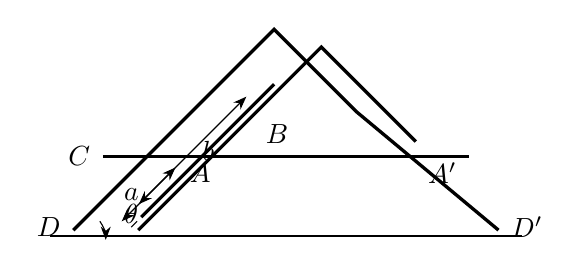
\begin{tikzpicture}[>=Stealth,scale=0.75]
  \draw[thick] (-4,0) -- (4,0);
  \draw[very thick] (-3.6,0.1) -- (-0.2,3.5) -- (1.2,2.1) -- (3.6,0.1);
  \draw[very thick] (-2.5,0.1) -- (0.6,3.2) -- (2.2,1.6);
  \draw[very thick] (-3.1,1.35) -- (3.1,1.35);
  \draw[very thick] (-2.45,0.32) -- (-0.2,2.57);
  \draw[dashed] (-2.62,0.15) -- (-0.37,2.40);
  \node[left] at (-3.65,0.15) {$D$}; \node[right] at (3.65,0.15) {$D'$};
  \node[left] at (-3.15,1.35) {$C$}; \node at (-1.45,1.06) {$A$};
  \node at (2.65,1.06) {$A'$}; \node at (-0.15,1.72) {$B$};
  \draw[<->] (-2.78,0.25) -- (-1.87,1.16) node[midway,left] {$a$};
  \draw[<->] (-2.49,0.54) -- (-0.67,2.36) node[midway,right] {$b$};
  \draw[->] (-3.15,0.25) arc[start angle=35,end angle=0,radius=0.55];
  \node at (-2.62,0.37) {$\theta$};
\end{tikzpicture}

\caption{第40届复赛第4题图4c的TikZ重绘：三单元编木拱桥侧视结构。}\label{fig:cpho40q04}
\end{figure}
\begin{enumerate}
\item 若 $D$ 杆下端至与 $A$ 杆接触点的长度为 $a$，求其至与 $B$ 杆接触点的长度 $b$。
\item 分析 $A,B,C,D$ 四杆受力，画出 $C,D$ 的受力图，并列出平衡方程。
\item 当 $M=6m$、$\theta=45^\circ$、$L=30\,\mathrm{cm}$、$a=16\,\mathrm{cm}$、$R=2(\sqrt2-1)\,\mathrm{cm}$ 时，求保持平衡的 $\mu,\mu'$ 条件。
\end{enumerate}
\subsection{参考解答整理}
\paragraph{（1）接触位置的几何关系。}圆柱杆接触的几何关系给出
\[b=a+4R\cot\frac\theta2.\]
\paragraph{（2）受力与平衡方程。} $C,D$ 两杆的受力关系以图\ref{fig:cpho40q04forces}表示。对 $A,B,C,D$ 分别列平衡条件，可写为
\[
N_1+mg=N_2\cos\theta+f_2\sin\theta,\quad
f_1+f_2\cos\theta=N_2\sin\theta,\quad f_1=f_2,
\]
\[N_3=2N_4\cos\theta+mg,\qquad 2N_1=N_3+Mg,
\]
\[
N_5+N_4\cos\theta=N_2\cos\theta+f_2\sin\theta+Mg,
\quad f_5+N_2\sin\theta=N_4\sin\theta+f_2\cos\theta.
\]
以 $D$ 杆与地面的接触点取力矩，
\[
N_2a+Mg\left(\frac L2\cos\theta-R\sin\theta\right)=N_4b+2Rf_2.
\]
\begin{figure}[htbp]\centering
\begin{tikzpicture}[>=Stealth,scale=0.72]
  \begin{scope}
    \draw[very thick] (-1.65,0) -- (1.65,0);
    \draw[thick] (-0.95,-0.36) circle (0.28);
    \draw[thick] (0.95,-0.36) circle (0.28);
    \draw[thick] (0,0.36) circle (0.28);
    \draw[->,thick] (-0.95,0) -- (-0.95,0.92) node[above] {$N_1$};
    \draw[->,thick] (0.95,0) -- (0.95,0.92) node[above] {$N_1$};
    \draw[->,thick] (-1.25,0) -- (-1.83,0) node[left] {$f_1$};
    \draw[->,thick] (1.25,0) -- (1.83,0) node[right] {$f_1$};
    \draw[->,thick] (0,0) -- (0,-0.88) node[right] {$N_3,\ Mg$};
    \node[below] at (0,-1.12) {$C$ 杆受力示意};
  \end{scope}
  \begin{scope}[xshift=4.3cm]
    \draw[thick] (-1.45,0) -- (1.45,0);
    \draw[very thick] (-0.82,0.08) -- (1.06,1.96);
    \draw[thick] (-0.35,0.56) circle (0.28);
    \draw[thick] (0.62,1.53) circle (0.28);
    \draw[->,thick] (-0.82,0.08) -- (-0.82,0.96) node[left] {$N_5$};
    \draw[->,thick] (-0.82,0.08) -- (-0.06,0.08) node[below] {$f_5$};
    \draw[->,thick] (-0.35,0.56) -- (0.10,0.11) node[right] {$N_2$};
    \draw[->,thick] (-0.82,0.08) -- (-1.28,-0.38) node[left] {$f_2$};
    \draw[->,thick] (0.62,1.53) -- (0.13,2.02) node[left] {$N_4$};
    \draw[->,thick] (0.10,1.00) -- (0.10,0.27) node[right] {$Mg$};
    \node[below] at (0,-0.62) {$D$ 杆受力示意};
  \end{scope}
\end{tikzpicture}

\caption{依据题解图4a、4b重绘的 $C$ 杆与 $D$ 杆受力示意。}\label{fig:cpho40q04forces}
\end{figure}
\paragraph{（3）代入数值。}先得 $b=24\,\mathrm{cm}$。由上述方程组，
\[N_1=10.427mg,\qquad f_1=f_2=4.733mg,\qquad N_5=\frac{21}{2}mg,\qquad f_5=2.194mg.\]
杆件接触处需满足 $f_1\leq\mu N_1$、$f_2\leq\mu N_2$，地面处需满足 $f_5\leq\mu'N_5$。因此保持平衡的条件为
\[\mu\geq0.454,\qquad \mu'\geq0.209.\]
\subsection{转写依据}
题干和解析分别依据 \texttt{CPHO40-Q04\_transcription\_v1.md} 与 \texttt{CPHO40-Q04\_formula\_check\_v1.csv}；图4a至4c及题解受力图的结构和力标注均据相应图件核对记录重绘。图4a、4b原为历史/实物照片，图册保留其结构信息并以TikZ示意替代照片，不嵌入原始图片。

% 题干转写：完成
% 解析转写：完成
% 图形核对：完成
\section{第40届复赛第7题：大气分层、声速与声波传播}

\subsection{题干}

大气层最底部是对流层，厚度约为 $10\,\mathrm{km}$；在对流层中，空气温度随高度升高而降低。对流层顶部之上约 $10\,\mathrm{km}$ 的范围内温度近似不随高度变化，称为同温层；同温层上方一定高度范围内温度随高度升高而升高，称为逆温层，如图\ref{fig:cpho40q07}所示。

\begin{figure}[htbp]
  \centering
  \begin{tikzpicture}[scale=0.86]
  \fill[blue!12] (0,0) circle (1.55);
  \fill[orange!12] (0,0) circle (2.12);
  \fill[gray!18] (0,0) circle (2.72);
  \fill[blue!55!black] (0,0) circle (1.18);
  \draw[thick] (0,0) circle (1.55);
  \draw[thick] (0,0) circle (2.12);
  \draw[thick] (0,0) circle (2.72);
  \node[white] at (0,0) {地球};
  \node[rotate=42] at (-1.60,1.38) {对流层};
  \node[rotate=42] at (-2.05,1.77) {同温层};
  \node[rotate=42] at (-2.50,2.18) {逆温层};
  \draw[->,thick] (3.2,-2.2) -- (3.2,2.6) node[above] {高度 $z$};
  \draw[thick,blue!70!black] (3.2,-1.6) -- (3.2,0.2) -- (4.35,1.05) -- (4.35,2.25);
  \node[align=left,anchor=west] at (4.5,1.60) {温度随高度：\\对流层降低\\同温层近似不变\\逆温层升高};
\end{tikzpicture}

  \caption{第40届复赛第7题图7a的TikZ重绘。}
  \label{fig:cpho40q07}
\end{figure}

\begin{enumerate}
  \item 将对流层温度变化视为理想气体缓慢绝热上升的结果。设地表温度为 $T_0$，空气摩尔质量为 $\mu$，$\gamma=C_p/C_V$ 为常数，普适气体常量为 $R$，重力加速度为 $g$。求温度 $T$ 与高度 $z$ 的关系。
  \item 已知气体声速满足 $v_s^2=(\mathrm dp/\mathrm d\rho)_{\mathrm{adiabatic}}$。求声速与温度的关系，并讨论三层大气中声速随高度的变化。
  \item 将层间界面近似为平面；对流层和逆温层温度均取 $-10\,{}^\circ\mathrm C$，同温层温度取 $-55\,{}^\circ\mathrm C$。同温层内声源发出的声波入射到界面时，判断不同入射角下的折射、反射与全反射情形。
  \item 将三层界面近似为同心球面，且对流层与逆温层温度相同并高于同温层温度。声源和探测气球均可处于对流层或同温层。忽略地面反射、可折射时的反射以及能量吸收，分别讨论四种位置组合下能否探测几千千米外的声音。已知地球半径 $R_e\simeq6371\,\mathrm{km}$。
\end{enumerate}

\subsection{参考解答整理}

\paragraph{（1）对流层温度。}
在高度 $z$ 处，理想气体密度为
\[
\rho(z)=\frac{p(z)\mu}{RT(z)}.
\]
对高度为 $\Delta z$、横截面积为 $A$ 的气体微元列静力平衡方程，取极限得到
\[
\frac{\mathrm dp}{\mathrm dz}=-\rho g,
\qquad
\frac{\mathrm d\ln p}{\mathrm dz}=-\frac{\mu g}{RT}.
\]
绝热关系 $pV^\gamma=\text{常量}$ 与理想气体状态方程给出
\[
0=-(\gamma-1)\frac{\mathrm d\ln p}{\mathrm dz}
+\gamma\frac{\mathrm d\ln T}{\mathrm dz}.
\]
因此
\[
\frac{\mathrm dT}{\mathrm dz}=-\frac{(\gamma-1)\mu g}{\gamma R},
\qquad
T(z)=T_0-\frac{(\gamma-1)\mu g}{\gamma R}z.
\]

\paragraph{（2）声速。}
绝热过程可写为 $p=C\rho^\gamma$，于是
\[
v_s^2=\left(\frac{\mathrm dp}{\mathrm d\rho}\right)_{\mathrm{adiabatic}}
=\gamma\frac{p}{\rho}=\frac{\gamma RT}{\mu},
\qquad
v_s=\sqrt{\frac{\gamma RT}{\mu}}.
\]
故对流层中声速随高度升高而降低；同温层中声速近似不变；逆温层中声速随高度升高而增大。

\paragraph{（3）平面分层下的折射与全反射。}
外层温度为 $T_o=263.15\,\mathrm K$，同温层温度为 $T_i=218.15\,\mathrm K$，因此
\[
\frac{v_o}{v_i}=\sqrt{\frac{T_o}{T_i}}
=\sqrt{\frac{263.15}{218.15}}\simeq1.098.
\]
以界面法线为基准，入射角为 $\theta_i$、折射角为 $\theta_o$，折射关系为
\[
\sin\theta_o=\frac{v_o}{v_i}\sin\theta_i.
\]
临界入射角为
\[
\theta_{im}=\arcsin\!\left(\frac{v_i}{v_o}\right)
\simeq65.6^\circ.
\]
当 $\theta_i<\theta_{im}$ 时存在折射光线，并可同时有反射；当 $\theta_i>\theta_{im}$ 时不存在实数折射角，声波在同温层内发生全反射。

\paragraph{（4）球面分层下的远距离传播。}
设对流层顶部高度 $h_1=10\,\mathrm{km}$，同温层顶部高度 $h_2=20\,\mathrm{km}$。声源和气球同在对流层时，无遮挡的最远传播距离为
\[
l_1=2\sqrt{(R_e+h_1)^2-R_e^2}
\simeq2\sqrt{2R_eh_1}\simeq714\,\mathrm{km},
\]
因此只能探测短距离声音。声源在对流层、气球在同温层时，传播距离不超过
\[
l_2=\sqrt{(R_e+h_2)^2-R_e^2}
+\sqrt{(R_e+h_1)^2-R_e^2}
\simeq862\,\mathrm{km},
\]
也不能探测远距离声音。

若声源和气球同在同温层，满足全反射条件的声波可在上下两个界面间多次反射并被限制在同温层中，因而可以传播到远距离。若声源在同温层、气球在对流层，声波必须折射进入对流层且不能被地球阻挡，距离同样受 $l_2$ 限制，故只能探测短距离声音。

\end{document}
